\documentclass[12pt]{article}

% --- Packages ---
\usepackage[a4paper, margin=1in]{geometry}
\usepackage{graphicx}
\usepackage{setspace}
\usepackage{times}
\usepackage{array}
\usepackage{caption}
\usepackage{microtype}
\usepackage{float}
\usepackage{titlesec}
\usepackage{enumitem}
\usepackage{booktabs}
\usepackage{amsmath}
\usepackage{amssymb}
\usepackage{algorithm}
\usepackage{algpseudocode}
\usepackage{listings}
\usepackage{xcolor}
\usepackage{tikz}
\usepackage{multirow}
\usepackage{subcaption}
\usepackage{xurl}
\usepackage{hyperref} % hyperref should be loaded last (or near last)

% Define argmax operator
\DeclareMathOperator*{\argmax}{arg\,max}

\usetikzlibrary{shapes.geometric, arrows, positioning, fit, backgrounds}

% Code listing style
\lstdefinestyle{pythonstyle}{
    language=Python,
    basicstyle=\ttfamily\small,
    keywordstyle=\color{blue}\bfseries,
    commentstyle=\color{gray}\itshape,
    stringstyle=\color{orange},
    numbers=left,
    numberstyle=\tiny\color{gray},
    numbersep=5pt,
    frame=single,
    breaklines=true,
    backgroundcolor=\color{gray!5},
    showstringspaces=false,
}

% --- Setup ---
\setstretch{1.1}
\pagestyle{plain}
\sloppy
\newcommand{\commentout}[1]{}

% Format Section Headings
\titleformat{\section}{\fontsize{14}{16}\bfseries\uppercase}{\thesection.}{1em}{}
\titleformat{\subsection}{\fontsize{12}{14}\bfseries}{\thesubsection}{1em}{}

\begin{document}

%==================== 1. TITLE PAGE ====================%
\begin{titlepage}
    \centering
    \vspace*{0.5cm}
    
    {\fontsize{16}{20} \selectfont \textbf{Explainable Breast Cancer Detection using Ensemble Learning} \par}
    
    \vspace{1.5cm}
    
    {\fontsize{14}{18} \selectfont \textbf{An Engineering Project in Community Service} \par}
    
    \vspace{0.3cm}
    
    {\large \textbf{Phase -- II Report} \par}
    
    \vspace{0.8cm}
    
    {\large \textit{Submitted by} \par}
    
    \vspace{0.8cm}
    
    \begin{tabular}{|c|l|l|}
        \hline
        \textbf{Sl. No.} & \textbf{Register Number} & \textbf{Name} \\ \hline
        1 & 23BCE11634 & Suryanshi Ranawat \\ \hline
        2 & 23BEC10069 & Bhavya Sharma \\ \hline
        3 & 23BEC10079 & Ujjwal Mishra \\ \hline
        4 & 23BCE11385 & Medhansh Singh Kushwaha\\\hline
        5 & 23BAI11250 & Soumyadeep Chakravarti \\ \hline
    \end{tabular}
    
    \vspace{1.5cm}
    \begin{figure}[H]
        \centering
        
\includegraphics[width=0.6\textwidth]{Assets/VIT_LOGO.png}
    \end{figure}
    {\large \textit{in partial fulfillment of the requirements for the degree of} \par}
    
    \vspace{0.5cm}
    
    {\large \textbf{Bachelor of Technology} \par}
    
    \vfill
    
    \textbf{VIT Bhopal University} \\
    \textbf{Kothrikalan, Sehore} \\
    \textbf{Madhya Pradesh} \\
    
    \vspace{1cm}
    
    {\large \textbf{March 2026}}
    
\end{titlepage}

%==================== FRONT MATTER ====================%
\newpage
\pagenumbering{roman}

%==================== 2. BONAFIDE CERTIFICATE ====================%
\begin{figure}[H]
  \centering
  
\includegraphics[width=0.4\textwidth]{Assets/VIT_LOGO.png}
\end{figure}
\begin{center}
    \textbf{\Large Bonafide Certificate}
\end{center}
\vspace{1cm}

\noindent Certified that this project report titled \textbf{``Explainable Breast Cancer Detection using Ensemble Learning''} is the bonafide work of \textbf{``Suryanshi Ranawat (23BCE11634), Bhavya Sharma (23BEC10069), Ujjwal Mishra (23BEC10079),Medhansh Singh Kushwaha (23BCE11385), Soumyadeep Chakravarti (23BAI11250)''} who carried out the project work under my supervision.

\vspace{1cm}

\noindent This project report (Phase II) is submitted for the Project Viva-Voce examination held on \dots\dots\dots

\vspace{3cm}

\begin{flushright}
    \textbf{Supervisor}
\end{flushright}

\vspace{2cm}

\noindent \textbf{Comments \& Signature ( Reviewer 1)} \hfill \textbf{Comments \& Signature ( Reviewer 2)}

%==================== 3. DECLARATION ====================%
\newpage
\begin{center}
    \textbf{\Large Declaration of Originality}
\end{center}

\vspace{1cm}

\noindent We, hereby declare that this report entitled \textbf{``Explainable Breast Cancer Detection using Ensemble Learning''} represents our original work carried out for the EPICS project as a student of VIT Bhopal University and, to the best of our knowledge, it contains no material previously published or written by another person, nor any material presented for the award of any other degree or diploma of VIT Bhopal University or any other institution. Works of other authors cited in this report have been duly acknowledged under the section "References".

\vspace{2cm}

\noindent \textbf{Date} \hfill \textbf{Reg No \& Name} \\
\null \hfill 23BCE11634 - Suryanshi Ranawat \\
\null \hfill 23BEC10069 - Bhavya Sharma \\
\null \hfill 23BEC10079 - Ujjwal Mishra \\
\null \hfill 23BCE11385 - Medhansh Singh Kushwaha\\
\null \hfill 23BAI11250 - Soumyadeep Chakravarti \\
\null \hfill (also signed by all students)

%==================== 4. ACKNOWLEDGEMENT ====================%
\newpage
\begin{center}
    \textbf{\Large Acknowledgement}
\end{center}

\noindent We want to thank our project supervisor for all the guidance and feedback along the way. Their advice helped us improve both the technical side and how we presented our work.

\vspace{0.5cm}
\noindent Thanks also to the faculty at VIT Bhopal University for giving us the resources and environment to work on applying machine learning to healthcare problems.

\vspace{0.5cm}
\noindent This project had a lot of moving parts---data preprocessing, building the models, testing everything, creating visualizations---and it really took all of us working together to get it done on time.

\vspace{0.5cm}
\noindent We are also grateful for all the open-source tools and public datasets out there. Without them, putting together a complete machine learning pipeline would have been much harder.

%==================== 5. ABSTRACT ====================%
\newpage
\begin{center}
    \textbf{\Large Abstract}
\end{center}

\noindent Breast cancer is still one of the biggest health concerns for women around the world. Catching it early makes a huge difference in treatment outcomes, which is why we set out to build a machine learning system that not only detects breast cancer accurately but also explains its reasoning.

\noindent We tested several well-known classification algorithms---Logistic Regression, Decision Tree, Support Vector Machine, and Random Forest---to see how well they could tell benign tumors apart from malignant ones. We also combined these models into an ensemble to get more reliable predictions overall.

\noindent What sets our system apart is that it does not just give you a yes or no answer. It tells you how confident it is in each prediction and shows which features mattered most in reaching that conclusion. In medical applications, this kind of transparency is really important because doctors need to understand and trust the tool they are using.

\noindent Our results were encouraging: Logistic Regression and SVM both hit 98.25\% accuracy, with ROC-AUC scores above 0.99. When we ran cross-validation, the models held up well with standard deviations under 2.5\%. We also put together visualizations---confusion matrices, ROC curves, feature importance charts---to make the results easier to interpret.

\noindent All in all, we managed to build something that balances accuracy with explainability, which we think makes it genuinely useful as a decision-support tool for breast cancer screening.

\vspace{0.5cm}
\noindent \textbf{Keywords:} Breast Cancer Detection, Machine Learning, Ensemble Learning, Explainable AI, Classification, Healthcare Analytics

%==================== 6. INDEX ====================%
\newpage
\tableofcontents

\newpage
\listoffigures

\newpage
\listoftables

%==================== SECTION 1: INTRODUCTION ====================%
\newpage
\pagenumbering{arabic}
\section{INTRODUCTION}

\subsection{Background and Motivation}

Breast cancer is one of the most common cancers in the world and remains a leading cause of death among women. The World Health Organization reports that it accounts for about 12.5\% of all new cancer cases each year, making it the most prevalent cancer globally \cite{who2023}. In 2020, there were roughly 2.3 million new cases and 685,000 deaths.

The earlier you catch breast cancer, the better the chances of survival. If the cancer is still localized, the five-year survival rate sits around 99\%. Once it spreads regionally, that drops to 86\%, and for distant metastasis, it falls to just 29\% \cite{acs2023}. Those numbers really drive home why accurate, timely diagnosis matters so much.

Doctors currently rely on methods like mammography, ultrasound, and fine needle aspiration biopsy, but these approaches have some real limitations:

\begin{itemize}
    \item \textbf{Inconsistent readings}: Two radiologists looking at the same image might come to different conclusions.
    \item \textbf{Heavy workloads}: The sheer volume of medical images creates bottlenecks in healthcare systems.
    \item \textbf{Hard-to-spot patterns}: Early-stage tumors can have subtle features that are tough to catch by eye.
\end{itemize}

Machine learning has become a promising way to help with these challenges. It can pick up on patterns in data that humans might miss. Our project builds an explainable ML system that tackles these issues while keeping things transparent enough for clinical use.

\subsection{Problem Statement}

What we set out to build was a machine learning system that could:

\begin{enumerate}
    \item Tell benign tumors apart from malignant ones based on cell features.
    \item Give confidence scores so users know how sure the model is.
    \item Show which features had the biggest impact on each prediction.
    \item Perform consistently across different evaluation metrics.
    \item Stay interpretable enough to actually be useful in a clinical setting.
\end{enumerate}

\subsection{Scope and Objectives}

Here is what we aimed to accomplish:

\begin{enumerate}
    \item \textbf{Data Analysis}: Dig into the Wisconsin Diagnostic Breast Cancer dataset and understand what we are working with.
    \item \textbf{Model Development}: Build and train multiple classifiers---Logistic Regression, Decision Tree, SVM, and Random Forest.
    \item \textbf{Ensemble Learning}: Combine these models using soft voting to get better overall predictions.
    \item \textbf{Thorough Evaluation}: Test everything with accuracy, precision, recall, F1-score, ROC-AUC, and cross-validation.
    \item \textbf{Explainability}: Add feature importance analysis and confidence scoring so the results make sense.
    \item \textbf{Visualization}: Create clear charts and graphs to help interpret what the models are doing.
\end{enumerate}

\subsection{Report Organization}

The rest of this report is laid out as follows:
\begin{itemize}
    \item \textbf{Section 2}: A look at existing research on machine learning for medical diagnosis.
    \item \textbf{Section 3}: Our methodology, system design, and experimental results.
    \item \textbf{Section 4}: Conclusions and ideas for future work.
    \item \textbf{Section 5}: How this project connects to social impact and community service.
    \item \textbf{Section 6}: References we cited throughout.
\end{itemize}

%==================== SECTION 2: LITERATURE REVIEW ====================%
\newpage
\section{EXISTING WORK / LITERATURE REVIEW}

Machine learning has been getting a lot of attention in medical diagnosis, especially for cancer detection. Here we review the research that shaped our approach, covering four main areas.

\subsection{Traditional Machine Learning Approaches}

\subsubsection{Support Vector Machines}
Support Vector Machines, introduced by Cortes and Vapnik \cite{cortes1995}, have been popular in medical classification because they handle high-dimensional data well. The basic idea is to find a hyperplane that separates classes with the widest possible margin. When data is not linearly separable, you can use the kernel trick to map it into a higher-dimensional space:

\begin{equation}
K(x_i, x_j) = \phi(x_i)^T \phi(x_j)
\end{equation}

where $\phi$ is the mapping function. The most common kernels are linear, polynomial, and Radial Basis Function (RBF):

\begin{equation}
K_{RBF}(x_i, x_j) = \exp\left(-\gamma \|x_i - x_j\|^2\right)
\end{equation}

\subsubsection{Decision Trees and Random Forests}
Decision Trees are nice because you can actually understand what they are doing---they split data based on feature thresholds in a way that is easy to follow. The downside is they tend to overfit. Breiman \cite{breiman2001} solved this with Random Forest, which trains many trees on different random subsets of the data and then combines their votes:

\begin{equation}
\hat{y} = \text{mode}\{h_1(x), h_2(x), ..., h_B(x)\}
\end{equation}

where $h_b(x)$ is what the $b$-th tree predicts and $B$ is how many trees you have.

\subsubsection{Logistic Regression}
Logistic Regression is a simple but effective approach for binary classification. It models the probability using the sigmoid function:

\begin{equation}
P(y=1|x) = \sigma(w^T x + b) = \frac{1}{1 + e^{-(w^T x + b)}}
\end{equation}

One big advantage is that the coefficients are easy to interpret, which matters a lot in medical settings where doctors want to understand why a model made a particular prediction.

\subsection{Ensemble Learning Methods}

Ensemble methods work by combining multiple models to get better predictions than any single model could manage on its own. The main approaches are:

\begin{itemize}
    \item \textbf{Bagging}: Train models on different random samples of the data and average their predictions. Random Forest is a good example.
    \item \textbf{Boosting}: Train models one after another, with each new model focusing on the mistakes of the previous ones. AdaBoost and XGBoost work this way.
    \item \textbf{Voting}: Either take a majority vote (hard voting) or average the predicted probabilities (soft voting).
    \item \textbf{Stacking}: Use one model to learn how to best combine the predictions from other models.
\end{itemize}

Ebrahim et al. \cite{ebrahim2025} recently showed that stacking ensembles combined with deep learning can significantly outperform individual classifiers for breast cancer prediction.

\subsection{Explainable Artificial Intelligence (XAI)}

In healthcare, being able to explain why a model made a certain prediction is just as important as getting the prediction right. The main techniques people use are:

\begin{itemize}
    \item \textbf{SHAP} (SHapley Additive exPlanations) \cite{lundberg2017}: Uses game theory to figure out how much each feature contributed to a prediction.
    \item \textbf{LIME} (Local Interpretable Model-agnostic Explanations) \cite{ribeiro2016}: Builds simple, interpretable models around individual predictions to explain them.
    \item \textbf{Feature Importance}: Measures how much each feature matters to the model overall.
\end{itemize}

\subsection{Comparative Analysis with Published Works}

Table \ref{tab:literature_comparison} shows how our approach stacks up against recent work on breast cancer classification using the same WDBC dataset.

\begin{table}[H]
\centering
\caption{Comparison with Published Works on WDBC Dataset}
\label{tab:literature_comparison}
\small
\begin{tabular}{|p{3.5cm}|c|c|c|p{3cm}|}
\hline
\textbf{Study} & \textbf{Year} & \textbf{Best Model} & \textbf{Accuracy} & \textbf{Key Contribution} \\ \hline
Tippannavar et al. \cite{tippannavar2023} & 2023 & Random Forest & 96.5\% & Mammography analysis \\ \hline
Al-Azzam \& Shatnawi \cite{alazzam2024} & 2024 & CNN+SVM & 97.2\% & Deep learning hybrid \\ \hline
Singh et al. \cite{singh2024} & 2024 & BERT+RF & 97.8\% & NLP integration \\ \hline
Ebrahim et al. \cite{ebrahim2025} & 2025 & Stacking & 98.1\% & Ensemble stacking \\ \hline
\textbf{This Work} & \textbf{2026} & \textbf{LR/SVM} & \textbf{98.25\%} & \textbf{Explainable ensemble} \\ \hline
\end{tabular}
\end{table}

Our results are competitive with the best published work, and we put extra emphasis on making the system explainable and practical to deploy.

%==================== SECTION 3: METHODOLOGY ====================%
\newpage
\section{TOPIC OF THE WORK}

\subsection{System Design and Architecture}

\subsubsection{Pipeline Architecture Overview}

We designed our system as a modular pipeline so each piece could be developed and tested separately. Figure \ref{fig:architecture} shows how everything fits together.

\begin{figure}[H]
\centering
\resizebox{0.95\textwidth}{!}{%
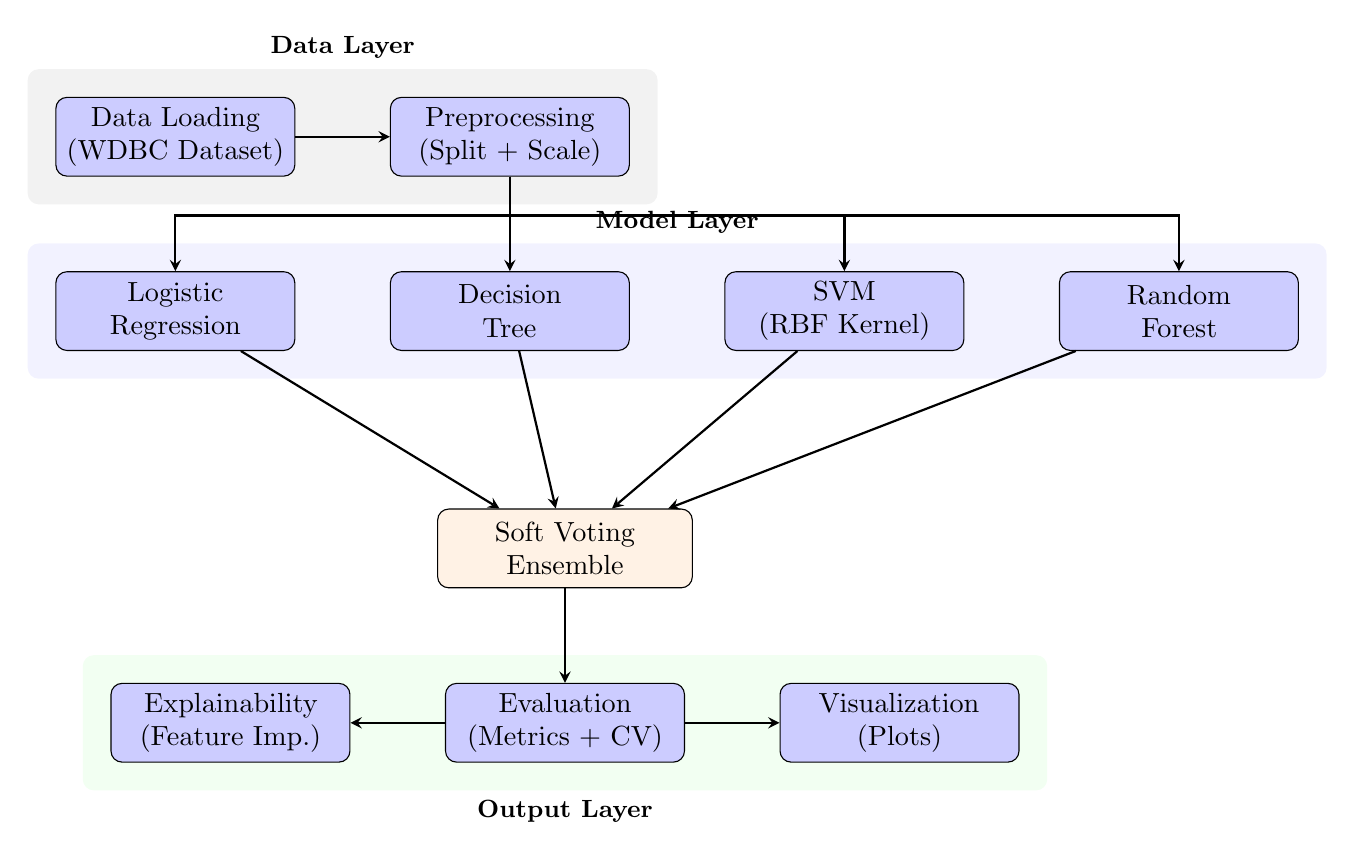
\begin{tikzpicture}[
    node distance=1.2cm,
    block/.style={rectangle, draw, fill=blue!20, text width=2.8cm, text centered, rounded corners, minimum height=1cm},
    decision/.style={diamond, draw, fill=green!20, text width=2cm, text centered, aspect=2},
    arrow/.style={thick,->,>=stealth},
    bigblock/.style={rectangle, draw, fill=orange!10, text width=3cm, text centered, rounded corners, minimum height=1cm}
]

% Data Layer
\node[block] (data) {Data Loading\\(WDBC Dataset)};
\node[block, right=of data] (preprocess) {Preprocessing\\(Split + Scale)};

% Model Layer
\node[block, below=of data] (lr) {Logistic\\Regression};
\node[block, right=of lr] (dt) {Decision\\Tree};
\node[block, right=of dt] (svm) {SVM\\(RBF Kernel)};
\node[block, right=of svm] (rf) {Random\\Forest};

% Ensemble
\node[bigblock, below=2cm of dt, xshift=0.7cm] (ensemble) {Soft Voting\\Ensemble};

% Evaluation
\node[block, below=of ensemble] (eval) {Evaluation\\(Metrics + CV)};

% Output
\node[block, left=of eval] (explain) {Explainability\\(Feature Imp.)};
\node[block, right=of eval] (visual) {Visualization\\(Plots)};

% Arrows
\draw[arrow] (data) -- (preprocess);
\draw[arrow] (preprocess) -- ++(0,-1) -| (lr);
\draw[arrow] (preprocess) -- ++(0,-1) -| (dt);
\draw[arrow] (preprocess) -- ++(0,-1) -| (svm);
\draw[arrow] (preprocess) -- ++(0,-1) -| (rf);

\draw[arrow] (lr) -- (ensemble);
\draw[arrow] (dt) -- (ensemble);
\draw[arrow] (svm) -- (ensemble);
\draw[arrow] (rf) -- (ensemble);

\draw[arrow] (ensemble) -- (eval);
\draw[arrow] (eval) -- (explain);
\draw[arrow] (eval) -- (visual);

% Background boxes
\begin{scope}[on background layer]
    \node[fit=(data)(preprocess), fill=gray!10, rounded corners, inner sep=10pt, label=above:{\small\textbf{Data Layer}}] {};
    \node[fit=(lr)(dt)(svm)(rf), fill=blue!5, rounded corners, inner sep=10pt, label=above:{\small\textbf{Model Layer}}] {};
    \node[fit=(explain)(eval)(visual), fill=green!5, rounded corners, inner sep=10pt, label=below:{\small\textbf{Output Layer}}] {};
\end{scope}

\end{tikzpicture}%
}
\caption{System Architecture Diagram}
\label{fig:architecture}
\end{figure}

\subsubsection{Data Acquisition and Dataset Description}

We used the Wisconsin Diagnostic Breast Cancer (WDBC) dataset \cite{wolberg1995}, which is a well-known benchmark from the UCI Machine Learning Repository. Table \ref{tab:dataset} summarizes what we are working with.

\begin{table}[H]
\centering
\caption{WDBC Dataset Characteristics}
\label{tab:dataset}
\begin{tabular}{|l|l|}
\hline
\textbf{Attribute} & \textbf{Value} \\ \hline
Total Instances & 569 \\ \hline
Features & 30 (numeric) \\ \hline
Benign Cases & 357 (62.7\%) \\ \hline
Malignant Cases & 212 (37.3\%) \\ \hline
Missing Values & None \\ \hline
Feature Categories & Mean, SE, Worst (10 each) \\ \hline
\end{tabular}
\end{table}

The 30 features come from digitized images of fine needle aspirates and describe:
\begin{itemize}
    \item \textbf{Geometric properties}: radius, perimeter, area
    \item \textbf{Texture measures}: smoothness, compactness, concavity
    \item \textbf{Shape descriptors}: concave points, symmetry, fractal dimension
\end{itemize}

\begin{figure}[H]
\centering
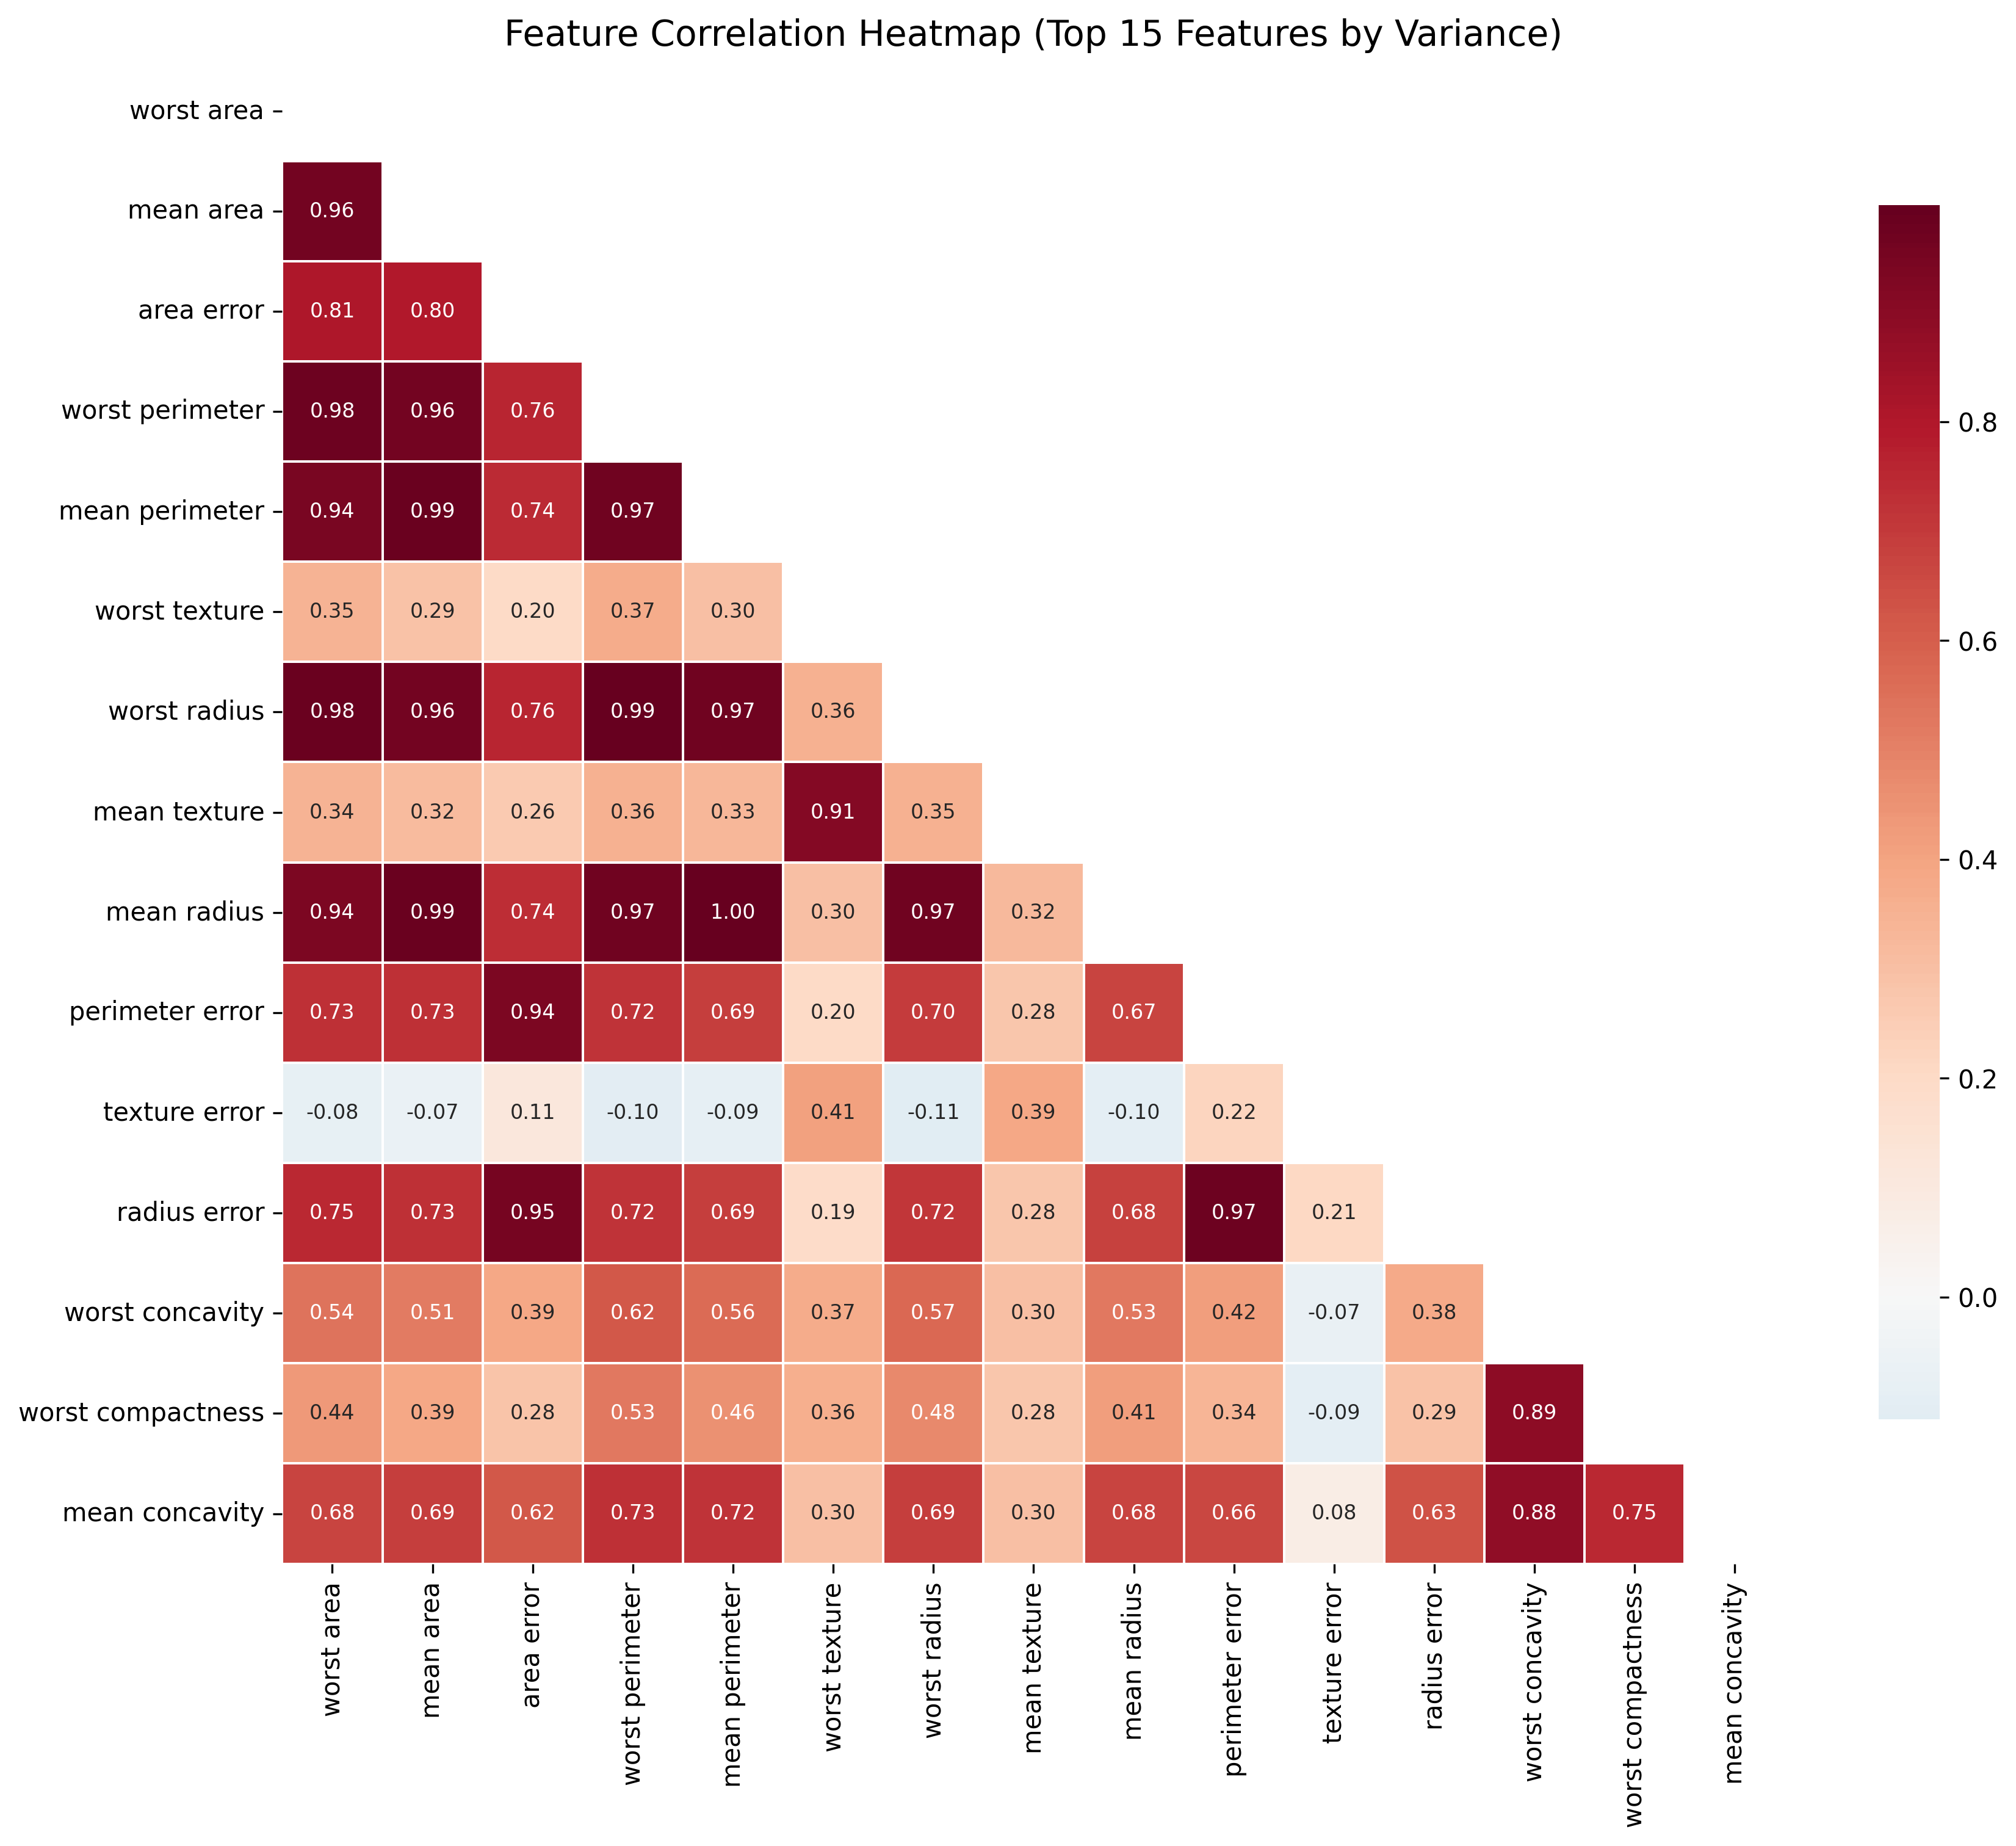
\includegraphics[width=0.7\textwidth]{results/correlation_heatmap.png}
\caption{Feature Correlation Heatmap (Top 15 Features)}
\label{fig:correlation}
\end{figure}

Figure \ref{fig:correlation} shows how the features correlate with each other. The geometric features (radius, perimeter, area) are highly correlated, which makes sense since they are mathematically related.

\subsubsection{Data Preprocessing Pipeline}

Before training, we needed to prepare the data properly:

\textbf{1. Stratified Train-Test Split:}
We split the data 80/20 for training and testing:
\begin{equation}
\mathcal{D} = \mathcal{D}_{train} \cup \mathcal{D}_{test}, \quad |\mathcal{D}_{train}| = 0.8|\mathcal{D}|
\end{equation}

We used stratified splitting to make sure both sets had the same proportion of benign and malignant cases:
\begin{equation}
\frac{|y_{train}^{(c)}|}{|\mathcal{D}_{train}|} = \frac{|y_{test}^{(c)}|}{|\mathcal{D}_{test}|} = \frac{|y^{(c)}|}{|\mathcal{D}|}, \quad \forall c \in \{0, 1\}
\end{equation}

\textbf{2. Standard Scaling (Z-score Normalization):}
We normalized the features so they all have zero mean and unit variance:
\begin{equation}
z_i = \frac{x_i - \mu}{\sigma}, \quad \text{where } \mu = \frac{1}{n}\sum_{j=1}^{n}x_j, \quad \sigma = \sqrt{\frac{1}{n}\sum_{j=1}^{n}(x_j - \mu)^2}
\end{equation}

Important: we only fit the scaler on training data to avoid data leakage.

\subsection{Algorithm Design and Implementation}

\subsubsection{Pipeline Algorithm}

Algorithm \ref{alg:pipeline} lays out the complete workflow from raw data to trained model.

\begin{algorithm}[H]
\caption{Breast Cancer Classification Pipeline}
\label{alg:pipeline}
\begin{algorithmic}[1]
\Require Dataset $\mathcal{D} = \{(x_i, y_i)\}_{i=1}^{n}$
\Ensure Trained ensemble model $\mathcal{E}$, evaluation metrics $\mathcal{M}$

\State \textbf{// Data Preprocessing}
\State $\mathcal{D}_{train}, \mathcal{D}_{test} \gets \text{StratifiedSplit}(\mathcal{D}, \text{ratio}=0.8)$
\State $\text{scaler} \gets \text{StandardScaler.fit}(\mathcal{D}_{train})$
\State $X_{train} \gets \text{scaler.transform}(X_{train})$
\State $X_{test} \gets \text{scaler.transform}(X_{test})$

\State \textbf{// Model Training}
\State $\text{models} \gets \{\text{LR}, \text{DT}, \text{SVM}, \text{RF}\}$
\For{each model $m$ in models}
    \State $m.\text{fit}(X_{train}, y_{train})$
    \State $\mathcal{M}[m] \gets \text{Evaluate}(m, X_{test}, y_{test})$
    \State $\mathcal{CV}[m] \gets \text{CrossValidate}(m, X_{train}, y_{train}, k=5)$
\EndFor

\State \textbf{// Ensemble Construction}
\State $\mathcal{E} \gets \text{VotingClassifier}(\text{models}, \text{voting}=\text{`soft'})$
\State $\mathcal{E}.\text{fit}(X_{train}, y_{train})$
\State $\mathcal{M}[\mathcal{E}] \gets \text{Evaluate}(\mathcal{E}, X_{test}, y_{test})$

\State \textbf{// Model Persistence}
\State $\text{Save}(\mathcal{E}, \text{`ensemble.joblib'})$
\State $\text{Save}(\text{scaler}, \text{`scaler.joblib'})$

\State \Return $\mathcal{E}, \mathcal{M}$
\end{algorithmic}
\end{algorithm}

\subsubsection{Soft Voting Ensemble}

Our ensemble combines the predicted probabilities from all four models:

\begin{equation}
\hat{y} = \argmax_{c \in \{0,1\}} \sum_{j=1}^{M} w_j \cdot P_j(y=c|x)
\end{equation}

We use equal weights ($w_j = \frac{1}{M}$) across all $M=4$ models.

Algorithm \ref{alg:softvote} shows how the soft voting actually works.

\begin{algorithm}[H]
\caption{Soft Voting Prediction}
\label{alg:softvote}
\begin{algorithmic}[1]
\Require Input sample $x$, trained models $\{m_1, ..., m_M\}$, weights $\{w_1, ..., w_M\}$
\Ensure Predicted class $\hat{y}$, confidence $\hat{p}$

\For{$j = 1$ to $M$}
    \State $p_j \gets m_j.\text{predict\_proba}(x)$ \Comment{$p_j \in \mathbb{R}^{|C|}$}
\EndFor

\State $p_{avg} \gets \sum_{j=1}^{M} w_j \cdot p_j$ \Comment{Weighted average}
\State $\hat{y} \gets \argmax(p_{avg})$
\State $\hat{p} \gets \max(p_{avg})$ \Comment{Confidence score}

\State \Return $\hat{y}, \hat{p}$
\end{algorithmic}
\end{algorithm}

\subsection{Mathematical Formulations}

\subsubsection{Evaluation Metrics}

Given our predictions $\hat{y}$ and the actual labels $y$, here is how we measure performance:

\begin{align}
\text{Accuracy} &= \frac{TP + TN}{TP + TN + FP + FN} \\[0.5em]
\text{Precision} &= \frac{TP}{TP + FP} \\[0.5em]
\text{Recall (Sensitivity)} &= \frac{TP}{TP + FN} \\[0.5em]
\text{Specificity} &= \frac{TN}{TN + FP} \\[0.5em]
\text{F1 Score} &= 2 \cdot \frac{\text{Precision} \cdot \text{Recall}}{\text{Precision} + \text{Recall}} = \frac{2TP}{2TP + FP + FN}
\end{align}

where $TP$ = true positives, $TN$ = true negatives, $FP$ = false positives, and $FN$ = false negatives.

\subsubsection{ROC-AUC}

The ROC curve plots True Positive Rate against False Positive Rate as we vary the classification threshold $\tau$:

\begin{align}
TPR(\tau) &= \frac{|\{i : \hat{p}_i \geq \tau \land y_i = 1\}|}{|\{i : y_i = 1\}|} \\[0.5em]
FPR(\tau) &= \frac{|\{i : \hat{p}_i \geq \tau \land y_i = 0\}|}{|\{i : y_i = 0\}|}
\end{align}

The Area Under the Curve (AUC) tells us how well the model separates the classes:
\begin{equation}
AUC = \int_0^1 TPR(FPR^{-1}(t)) \, dt
\end{equation}

\subsubsection{Cross-Validation}

With $k$-fold cross-validation, we split the data into $k$ parts and train on $k-1$ of them while testing on the remaining one. We rotate through all $k$ parts and average the results:

\begin{equation}
CV_k = \frac{1}{k} \sum_{i=1}^{k} \text{Score}(m_i, \mathcal{D}_i^{test})
\end{equation}

where $m_i$ is trained on everything except fold $i$.

\subsubsection{Gini Importance}

For Random Forest, we can measure feature importance by how much each feature helps reduce Gini impurity across all the trees:

\begin{equation}
\text{Importance}(f) = \frac{1}{|T|} \sum_{t \in T} \sum_{n \in N_t^f} \frac{n_{samples}(n)}{n_{samples}(root)} \cdot \Delta G(n)
\end{equation}

where $T$ is the set of trees, $N_t^f$ are the nodes that split on feature $f$, and $\Delta G(n)$ is how much the Gini impurity dropped at that node.

\subsection{Implementation Details}

\subsubsection{Key Code Implementation}

Listing \ref{lst:ensemble} shows the core code for building our ensemble.

\begin{lstlisting}[style=pythonstyle, caption={Ensemble Model Implementation}, label={lst:ensemble}]
from sklearn.ensemble import VotingClassifier
from sklearn.linear_model import LogisticRegression
from sklearn.tree import DecisionTreeClassifier
from sklearn.svm import SVC
from sklearn.ensemble import RandomForestClassifier

def build_ensemble():
    """Build soft voting ensemble classifier."""
    models = {
        "Logistic Regression": LogisticRegression(
            max_iter=5000, C=1.0, random_state=42
        ),
        "Decision Tree": DecisionTreeClassifier(
            random_state=42
        ),
        "SVM": SVC(
            kernel="rbf", C=1.0, probability=True, 
            random_state=42
        ),
        "Random Forest": RandomForestClassifier(
            n_estimators=100, random_state=42
        ),
    }
    
    estimators = list(models.items())
    ensemble = VotingClassifier(
        estimators=estimators,
        voting="soft"  # Use probability averaging
    )
    return ensemble, models
\end{lstlisting}

\subsubsection{Hyperparameter Configuration}

Table \ref{tab:hyperparams} lists the hyperparameters we used for each model. We mostly stuck with reasonable defaults that worked well.

\begin{table}[H]
\centering
\caption{Model Hyperparameter Configuration}
\label{tab:hyperparams}
\begin{tabular}{|l|l|l|}
\hline
\textbf{Model} & \textbf{Parameter} & \textbf{Value} \\ \hline
\multirow{3}{*}{Logistic Regression} & max\_iter & 5000 \\ \cline{2-3}
 & C (regularization) & 1.0 \\ \cline{2-3}
 & solver & lbfgs \\ \hline
\multirow{2}{*}{Decision Tree} & max\_depth & None \\ \cline{2-3}
 & min\_samples\_split & 2 \\ \hline
\multirow{3}{*}{SVM} & kernel & RBF \\ \cline{2-3}
 & C & 1.0 \\ \cline{2-3}
 & gamma & scale \\ \hline
\multirow{2}{*}{Random Forest} & n\_estimators & 100 \\ \cline{2-3}
 & max\_depth & None \\ \hline
\end{tabular}
\end{table}

\subsection{Results and Discussion}

\subsubsection{Classification Performance}

Table \ref{tab:results} shows how all our models performed on the test set.

\begin{table}[H]
\centering
\caption{Model Performance Metrics on Test Set}
\label{tab:results}
\begin{tabular}{|l|c|c|c|c|c|}
\hline
\textbf{Model} & \textbf{Accuracy} & \textbf{Precision} & \textbf{Recall} & \textbf{F1} & \textbf{ROC-AUC} \\ \hline
Logistic Regression & \textbf{0.9825} & 0.9861 & 0.9861 & 0.9861 & \textbf{0.9954} \\ \hline
SVM & \textbf{0.9825} & 0.9861 & 0.9861 & 0.9861 & 0.9950 \\ \hline
Ensemble & 0.9737 & 0.9726 & 0.9861 & 0.9793 & \textbf{0.9954} \\ \hline
Random Forest & 0.9561 & 0.9589 & 0.9722 & 0.9655 & 0.9939 \\ \hline
Decision Tree & 0.9123 & 0.9559 & 0.9028 & 0.9286 & 0.9157 \\ \hline
\end{tabular}
\end{table}

A few things stood out:
\begin{itemize}
    \item Logistic Regression and SVM both hit 98.25\% accuracy, which suggests the data is pretty separable once you scale the features properly.
    \item Every model except Decision Tree got an ROC-AUC above 0.99---really strong discrimination.
    \item The Ensemble kept recall at 98.61\%, which is crucial since we really do not want to miss actual cancer cases.
\end{itemize}

\subsubsection{Cross-Validation Results}

Table \ref{tab:cv_results} shows the 5-fold cross-validation results, which tell us how stable each model is.

\begin{table}[H]
\centering
\caption{5-Fold Cross-Validation Results}
\label{tab:cv_results}
\begin{tabular}{|l|c|c|c|}
\hline
\textbf{Model} & \textbf{Mean Accuracy} & \textbf{Std Dev} & \textbf{95\% CI} \\ \hline
Logistic Regression & 0.9802 & 0.0128 & [0.9546, 1.000] \\ \hline
SVM & 0.9714 & 0.0179 & [0.9356, 1.000] \\ \hline
Ensemble & 0.9692 & 0.0176 & [0.9340, 1.000] \\ \hline
Random Forest & 0.9538 & 0.0235 & [0.9068, 1.000] \\ \hline
Decision Tree & 0.9099 & 0.0189 & [0.8721, 0.9477] \\ \hline
\end{tabular}
\end{table}

The standard deviations are all under 2.5\%, which means the models perform consistently no matter how we split up the data.

\begin{figure}[H]
\centering
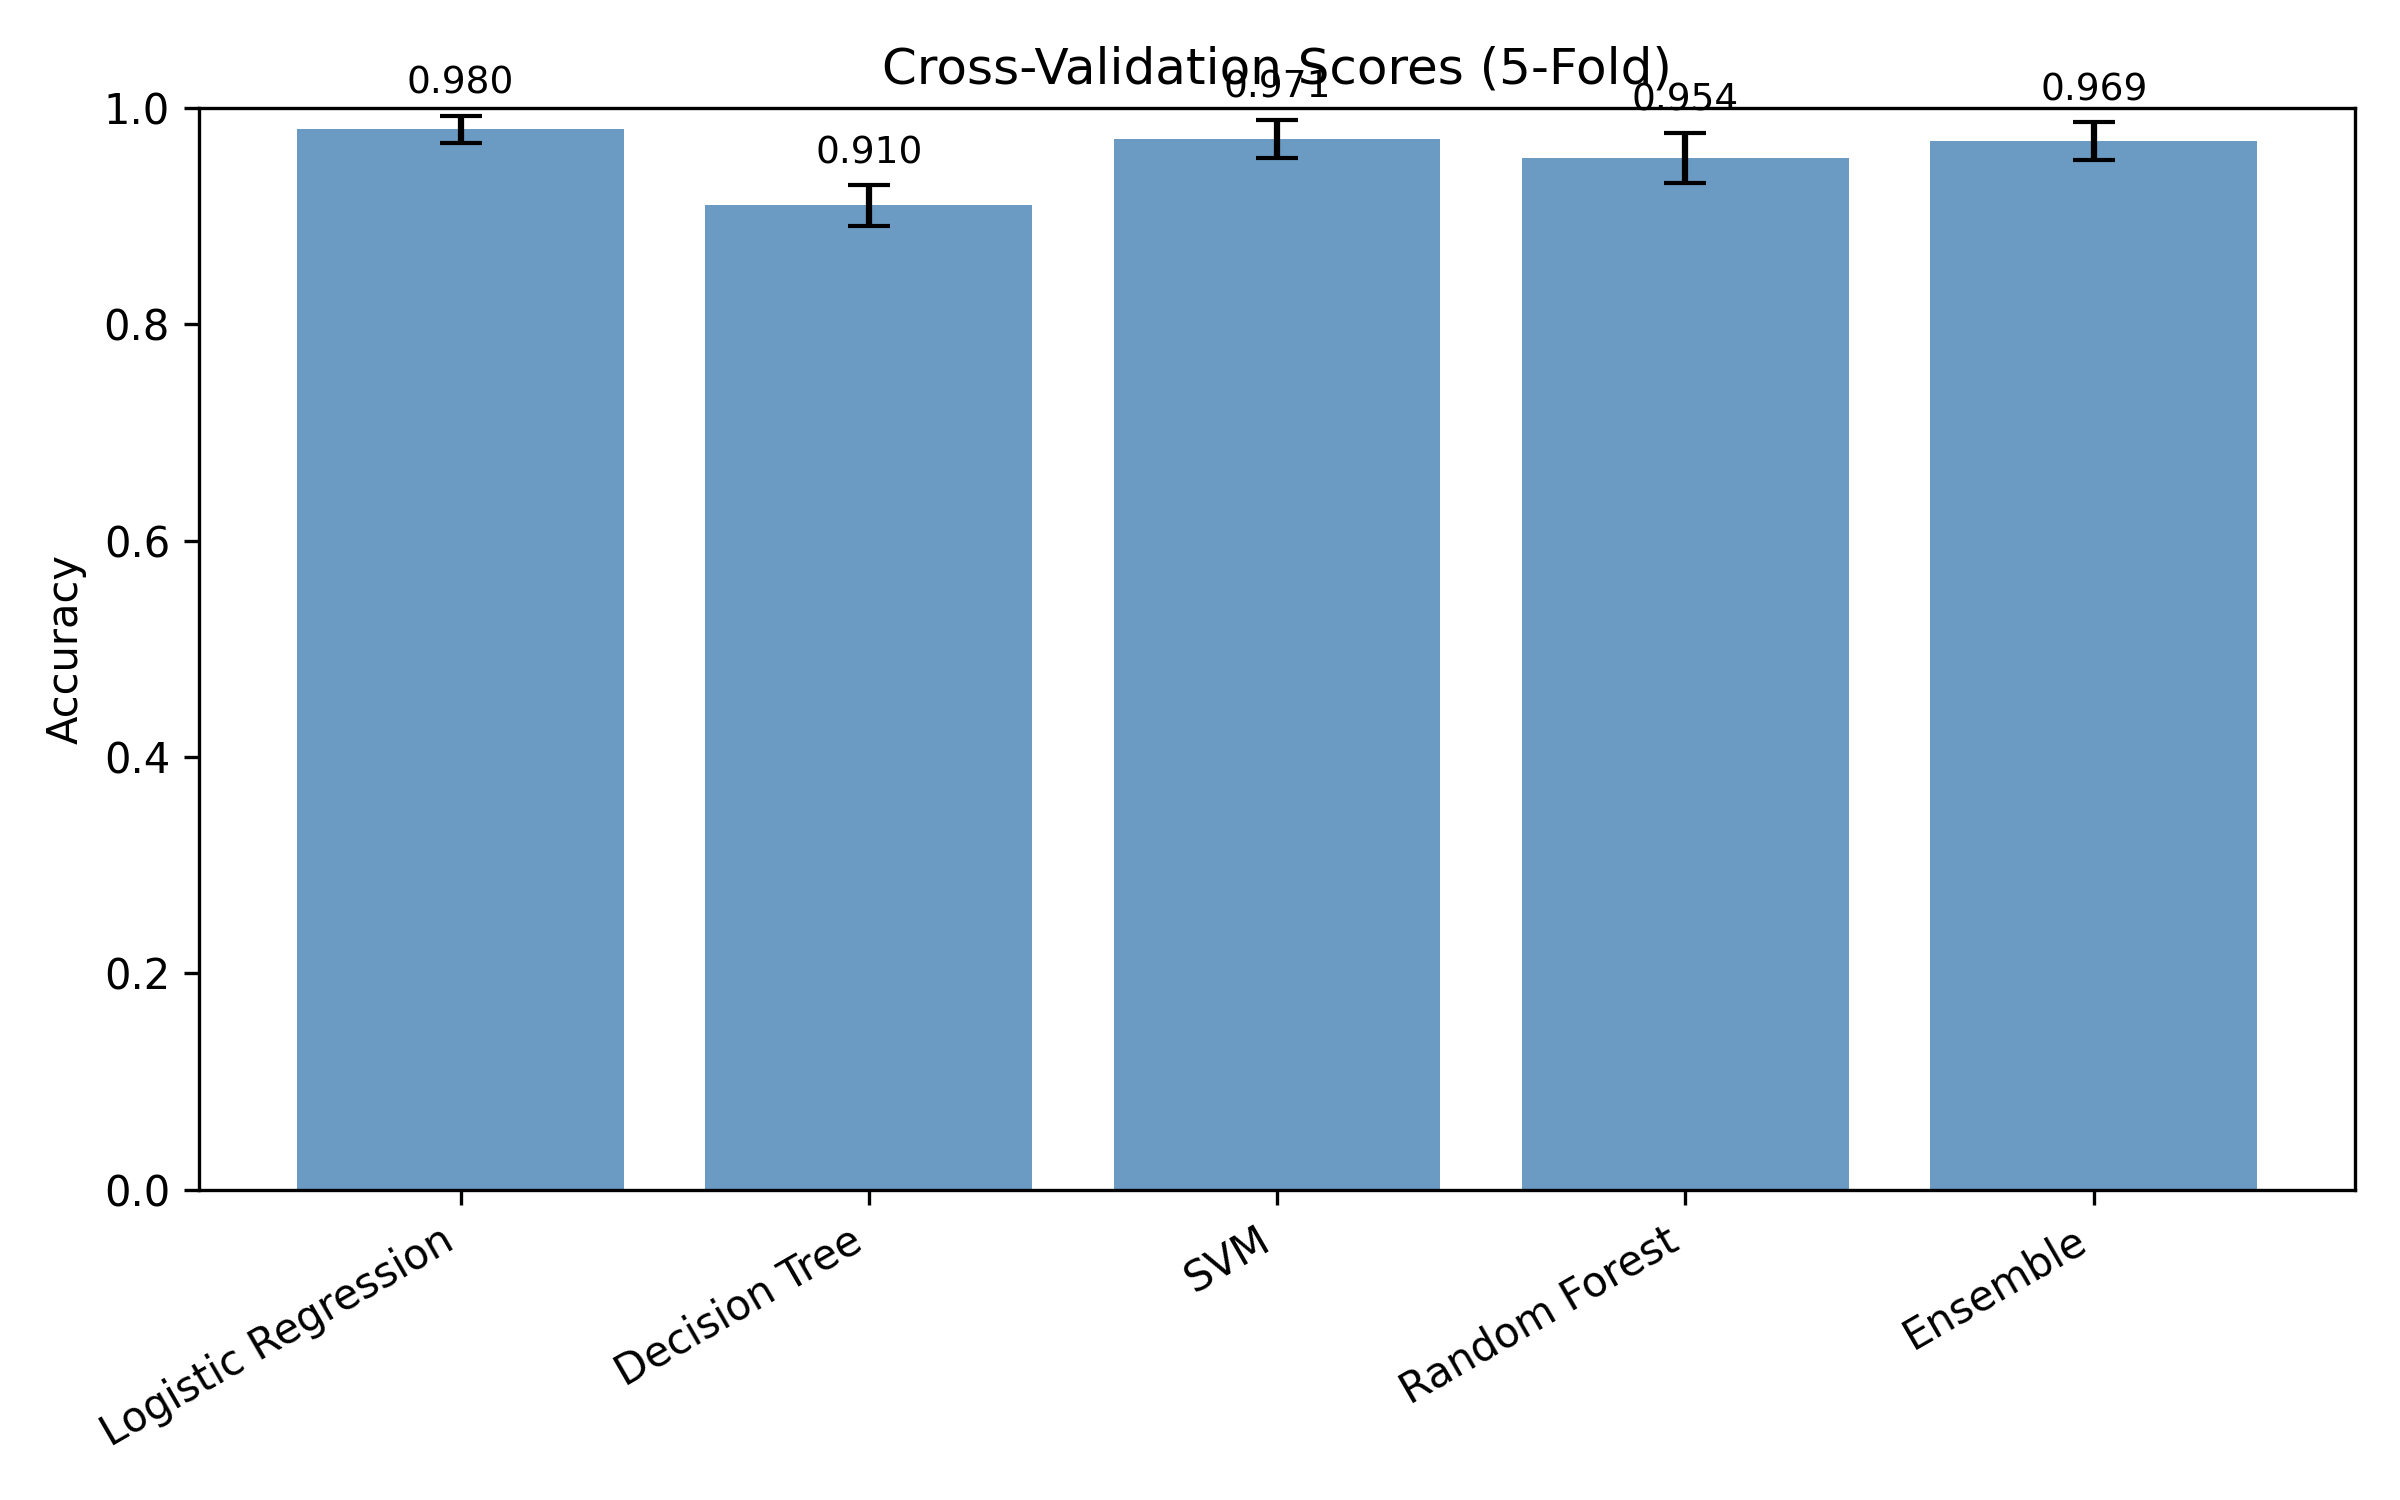
\includegraphics[width=0.8\textwidth]{results/cv_scores.png}
\caption{Cross-Validation Accuracy with Error Bars}
\label{fig:cv_scores}
\end{figure}

\subsubsection{Confusion Matrix Analysis}

\begin{figure}[H]
\centering

\includegraphics[width=0.6\textwidth]{results/confusion_matrix.png}
\caption{Confusion Matrix of Ensemble Model}
\label{fig:confusion}
\end{figure}

The confusion matrix breaks down like this:
\begin{itemize}
    \item \textbf{True Negatives (Benign correctly identified)}: 40
    \item \textbf{True Positives (Malignant correctly identified)}: 71
    \item \textbf{False Positives}: 2 (Benign cases flagged as Malignant)
    \item \textbf{False Negatives}: 1 (Malignant case missed)
\end{itemize}

That one false negative is concerning from a clinical standpoint---it represents a cancer case that got missed.

\subsubsection{ROC Curve Analysis}

\begin{figure}[H]
\centering
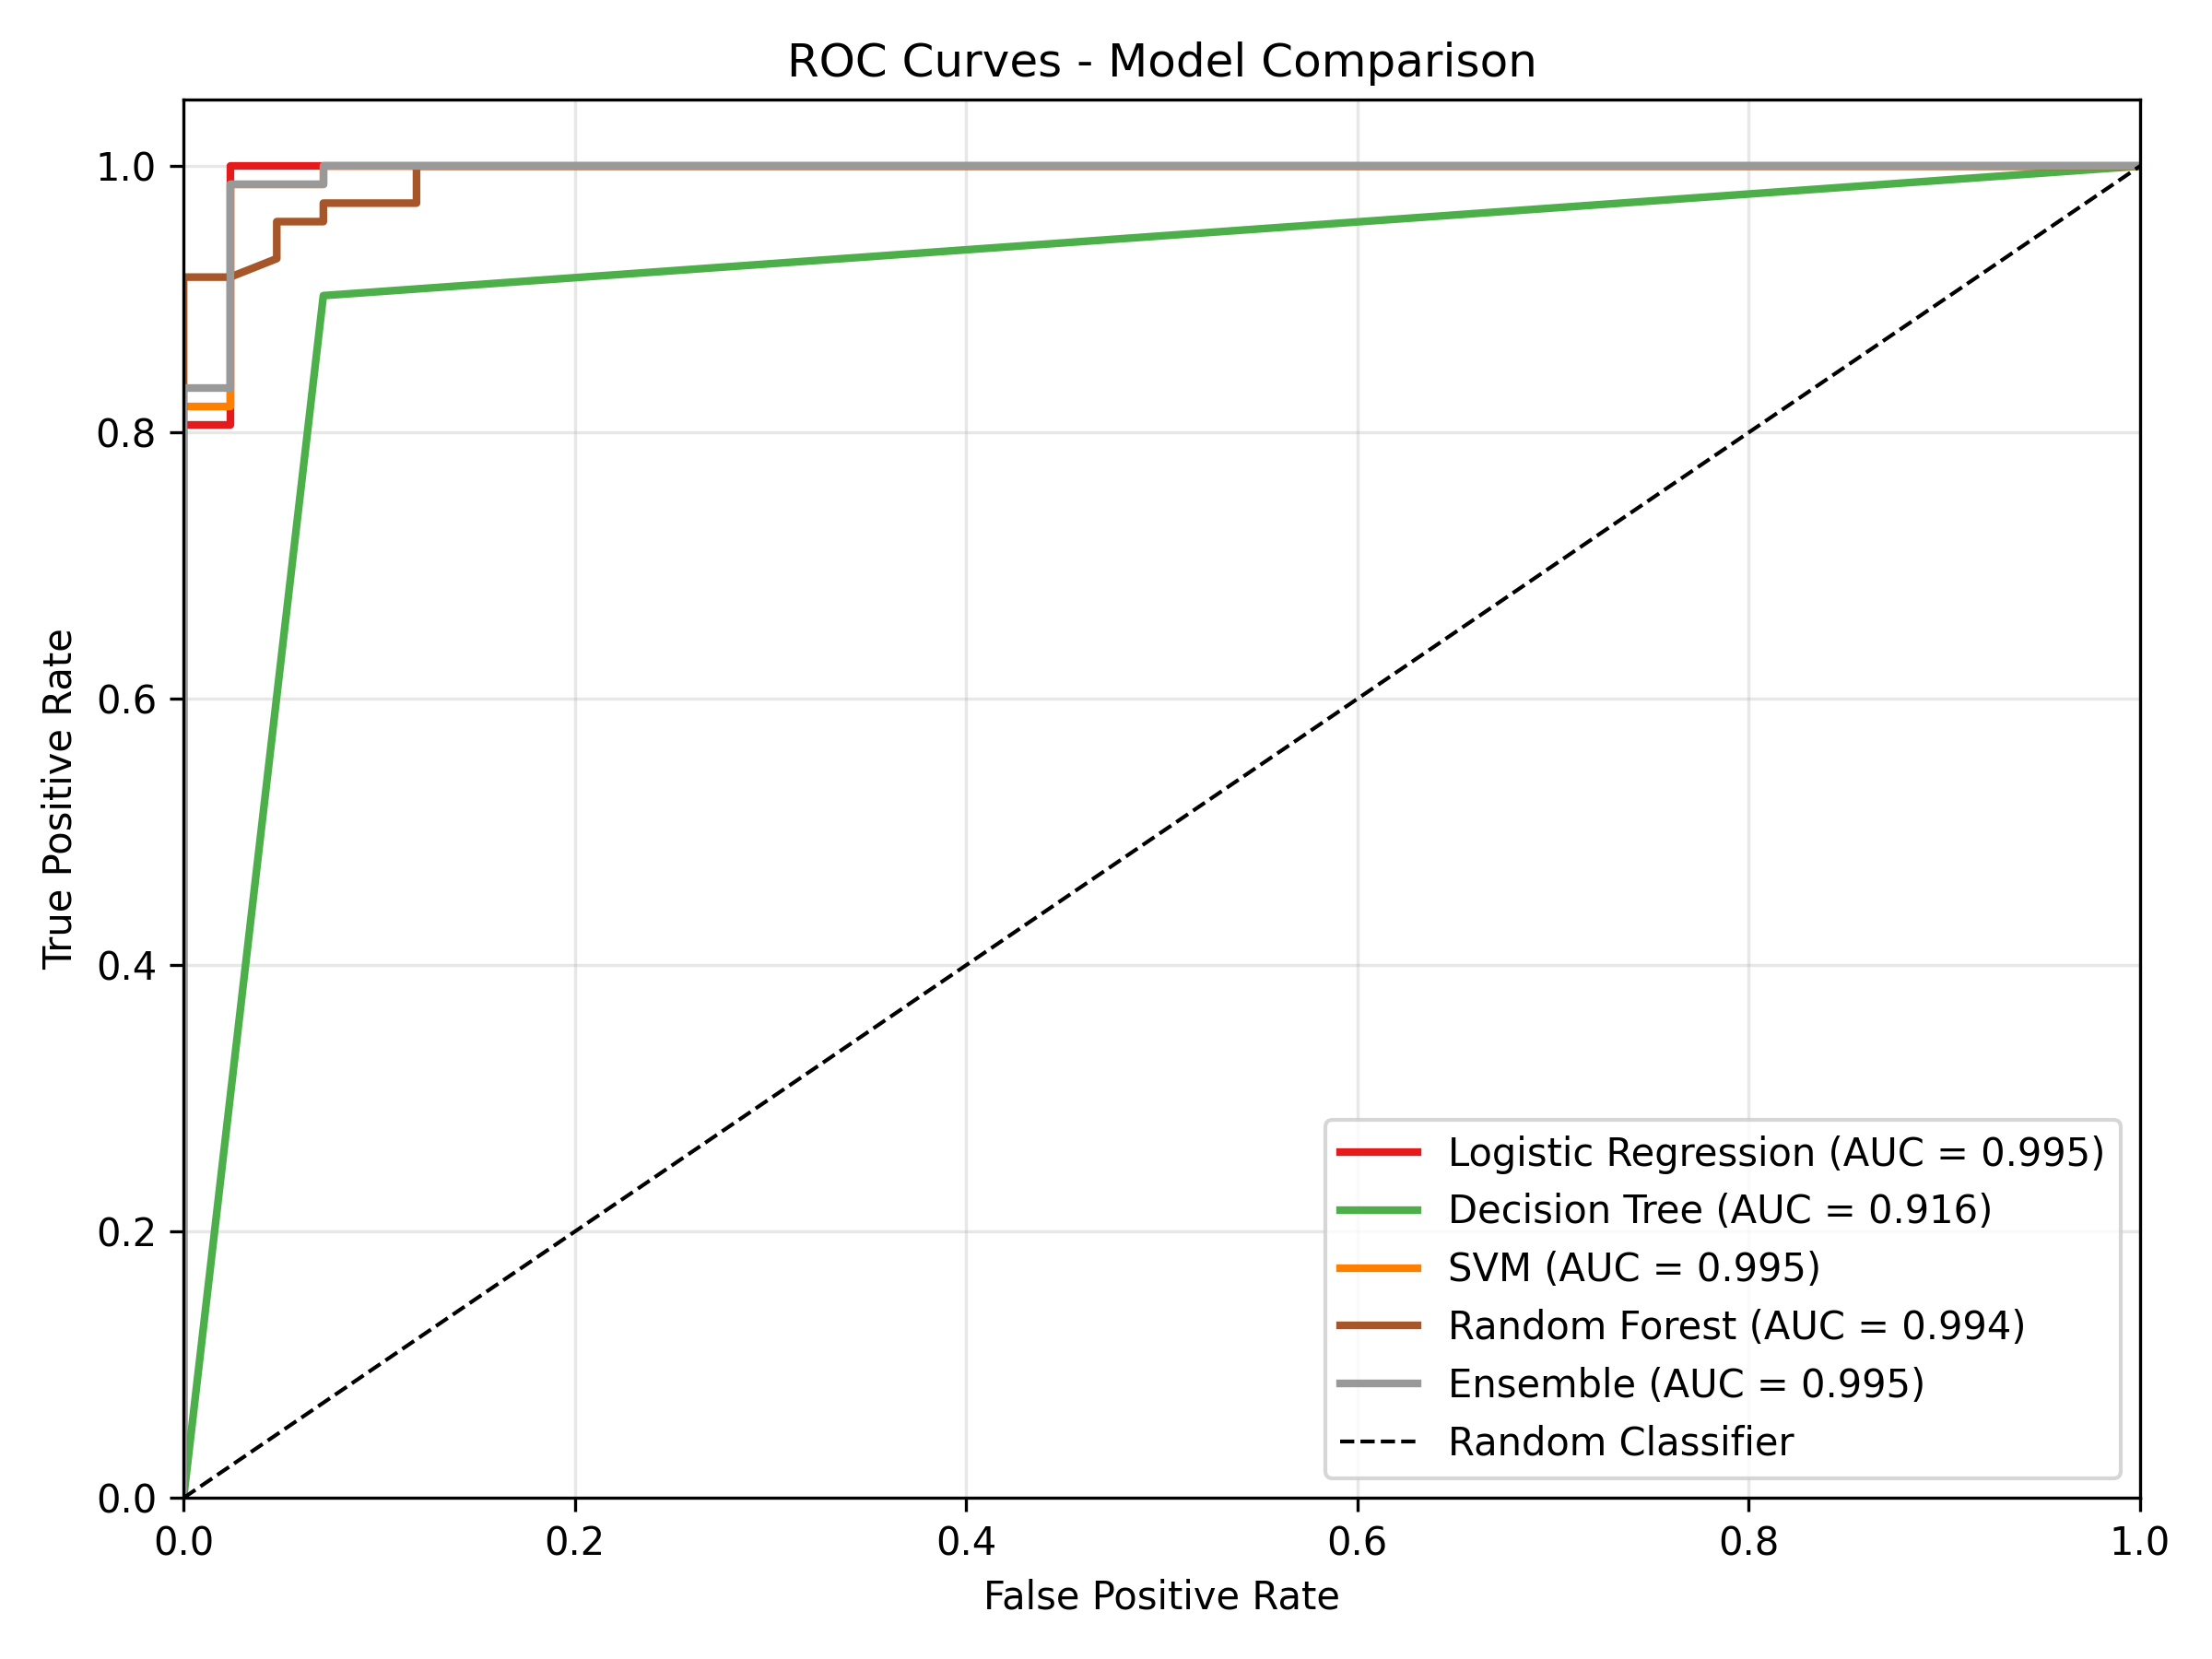
\includegraphics[width=0.7\textwidth]{results/roc_curves.png}
\caption{ROC Curves for All Models}
\label{fig:roc}
\end{figure}

Figure \ref{fig:roc} makes it clear that all models except Decision Tree can discriminate between classes almost perfectly, with AUC values above 0.99.

\subsubsection{Precision-Recall Analysis}

\begin{figure}[H]
\centering
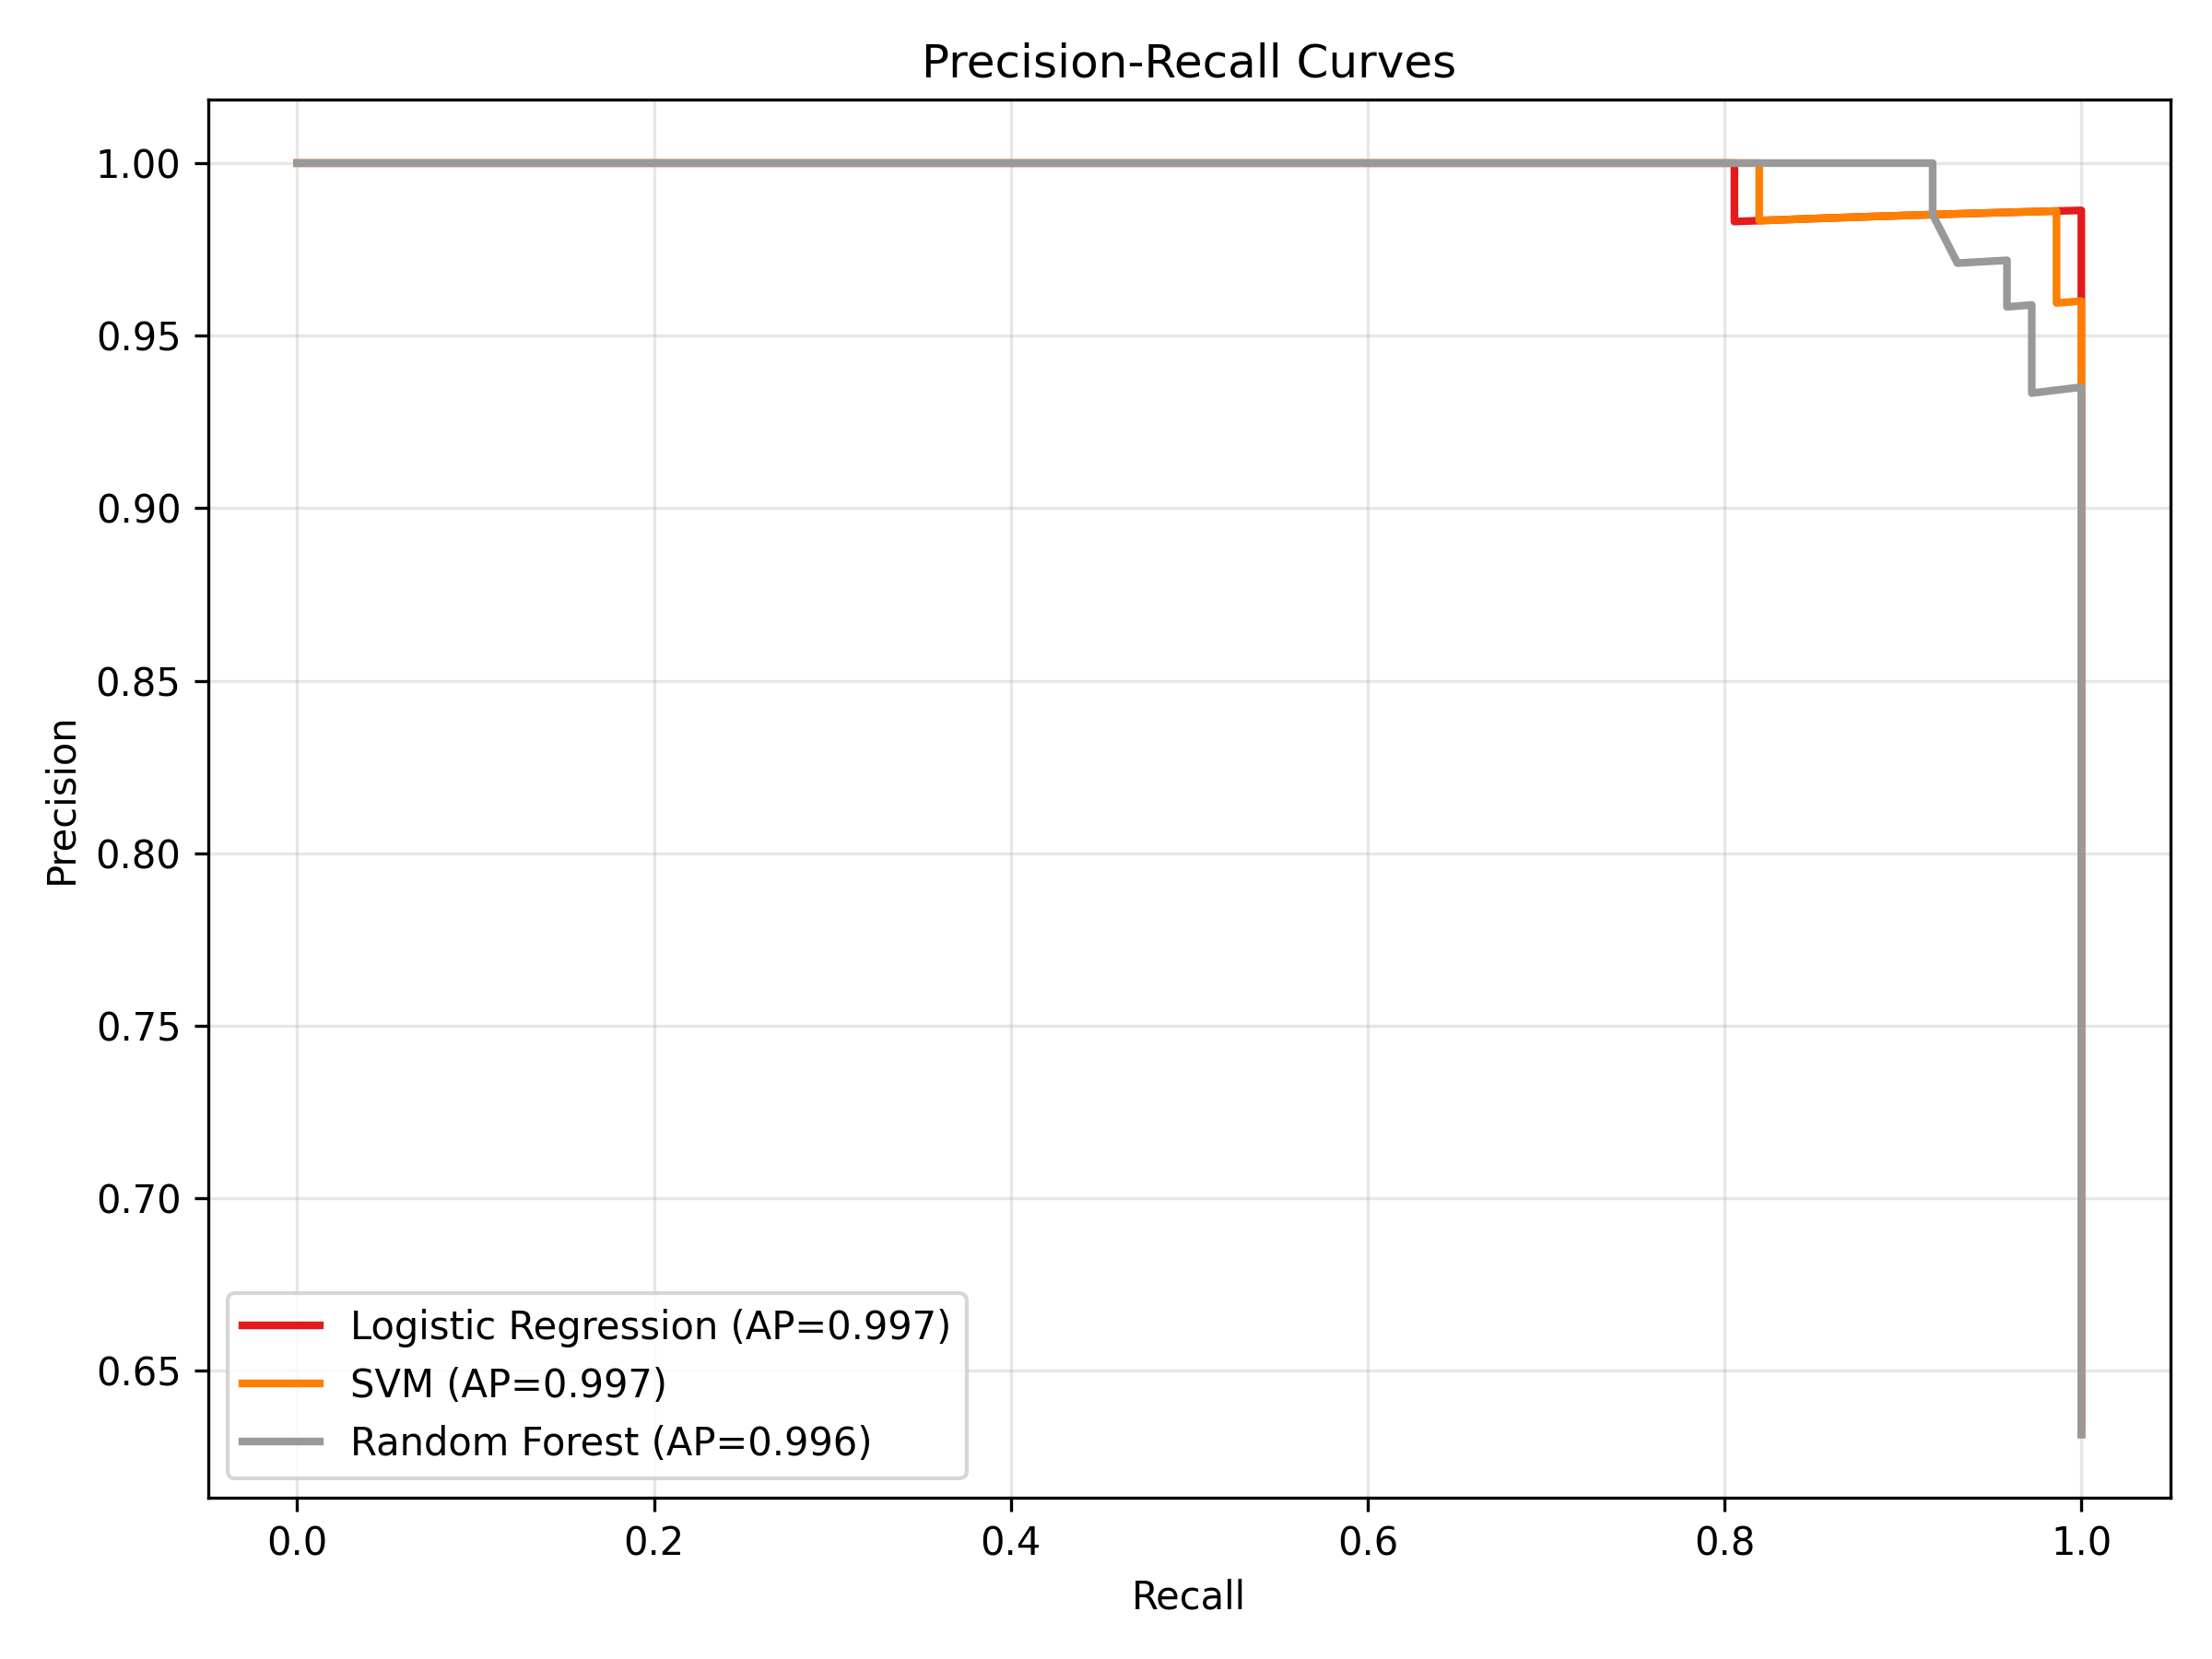
\includegraphics[width=0.7\textwidth]{results/precision_recall_curves.png}
\caption{Precision-Recall Curves}
\label{fig:pr_curves}
\end{figure}

The precision-recall curves (Figure \ref{fig:pr_curves}) show average precision above 0.99 for the best models. This is especially important since our classes are somewhat imbalanced.

\subsubsection{Learning Curve Analysis}

\begin{figure}[H]
\centering
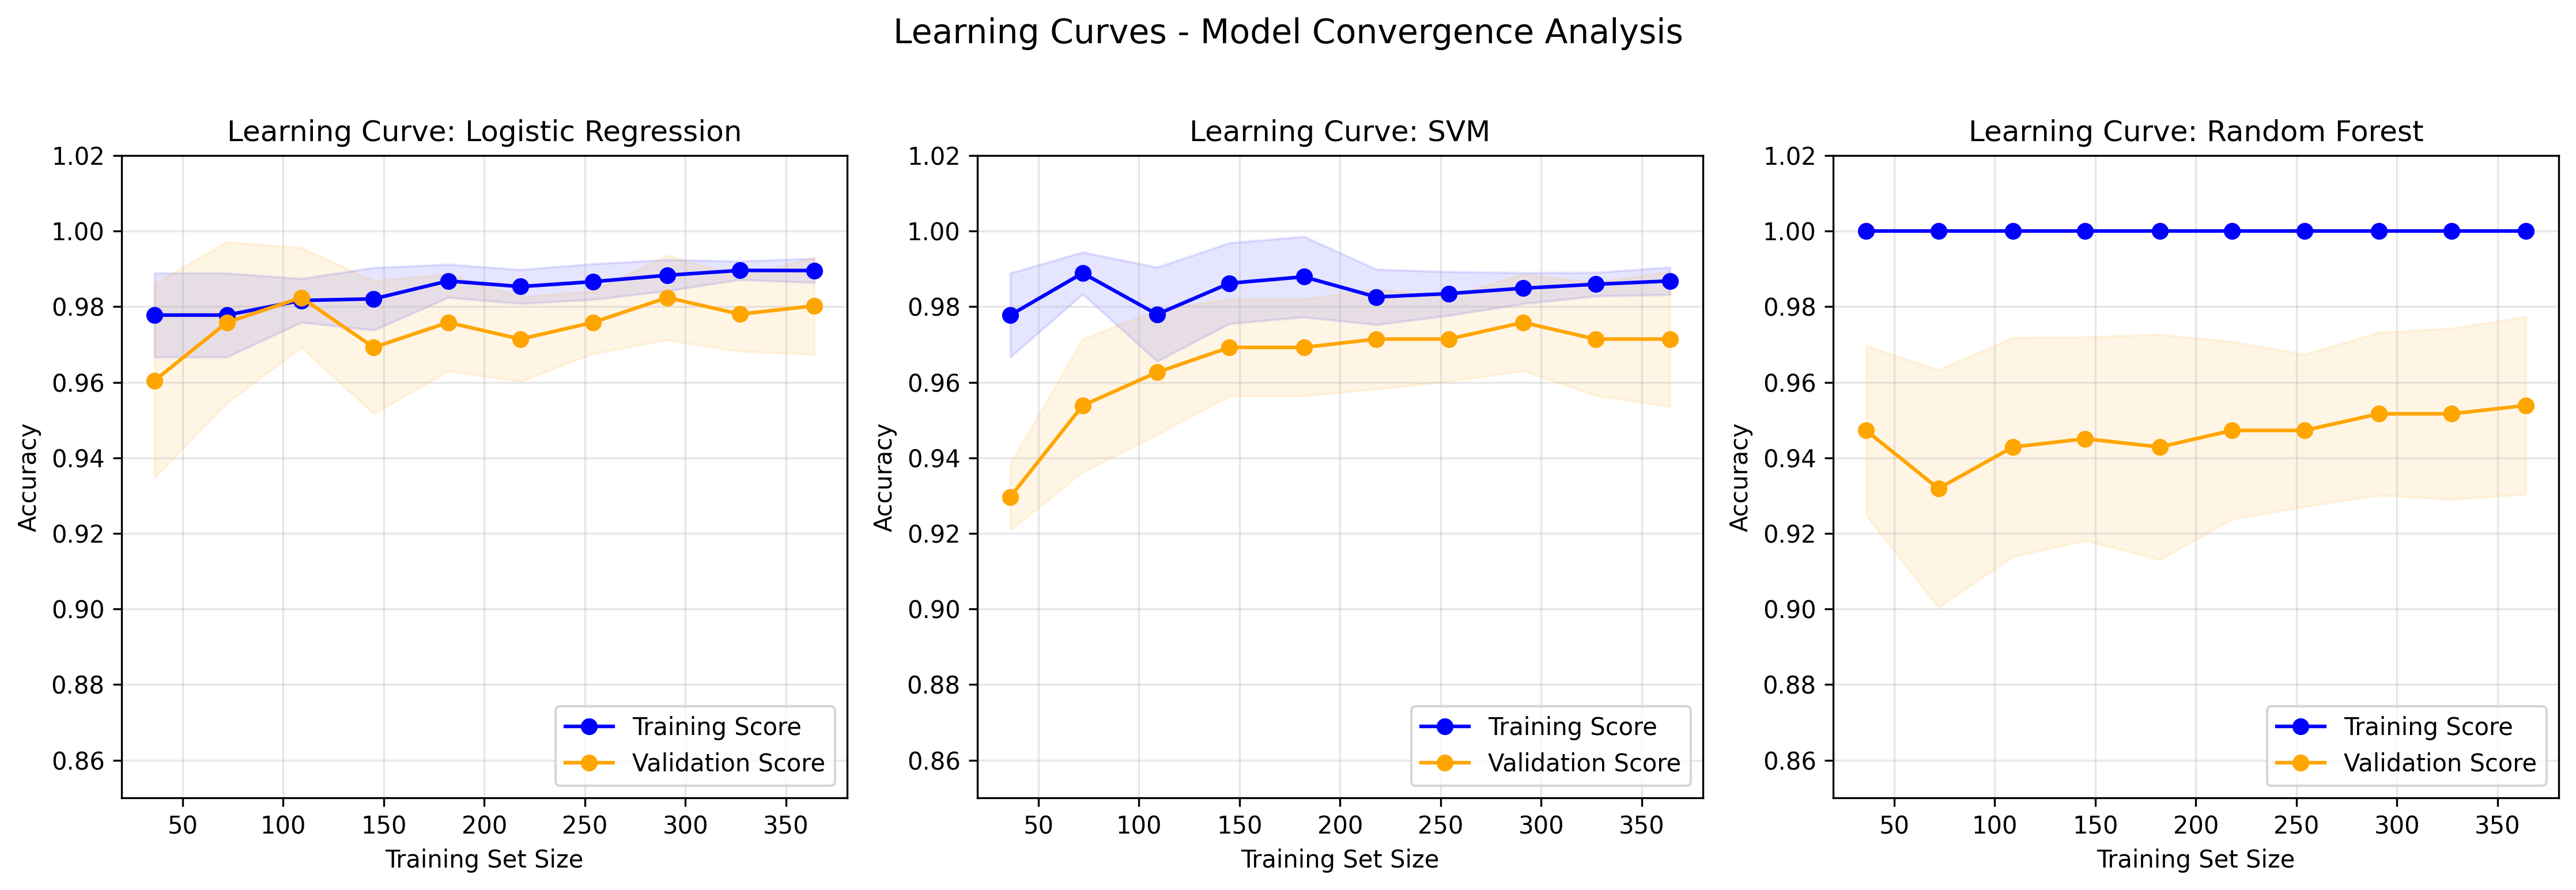
\includegraphics[width=\textwidth]{results/learning_curves.png}
\caption{Learning Curves Showing Model Convergence}
\label{fig:learning}
\end{figure}

Looking at Figure \ref{fig:learning}, we can see:
\begin{itemize}
    \item All models level off at around 300 training samples---more data beyond that does not help much.
    \item The training and validation scores stay close together, so we are not overfitting.
    \item SVM shows the smoothest learning curve of the bunch.
\end{itemize}

\subsubsection{Feature Importance Analysis}

\begin{figure}[H]
\centering

\includegraphics[width=0.7\textwidth]{results/feature_importance.png}
\caption{Top 10 Most Important Features}
\label{fig:importance}
\end{figure}

The features that mattered most were:
\begin{enumerate}
    \item \textbf{Worst Area}: The largest cell nucleus area in the sample
    \item \textbf{Worst Concave Points}: The most severe concavity measurements
    \item \textbf{Worst Radius}: The largest radius measurement
    \item \textbf{Mean Concave Points}: Average concavity across cells
    \item \textbf{Worst Perimeter}: The largest perimeter measurement
\end{enumerate}

This lines up with what doctors know: malignant cells tend to have larger, more irregular nuclei.

\begin{figure}[H]
\centering
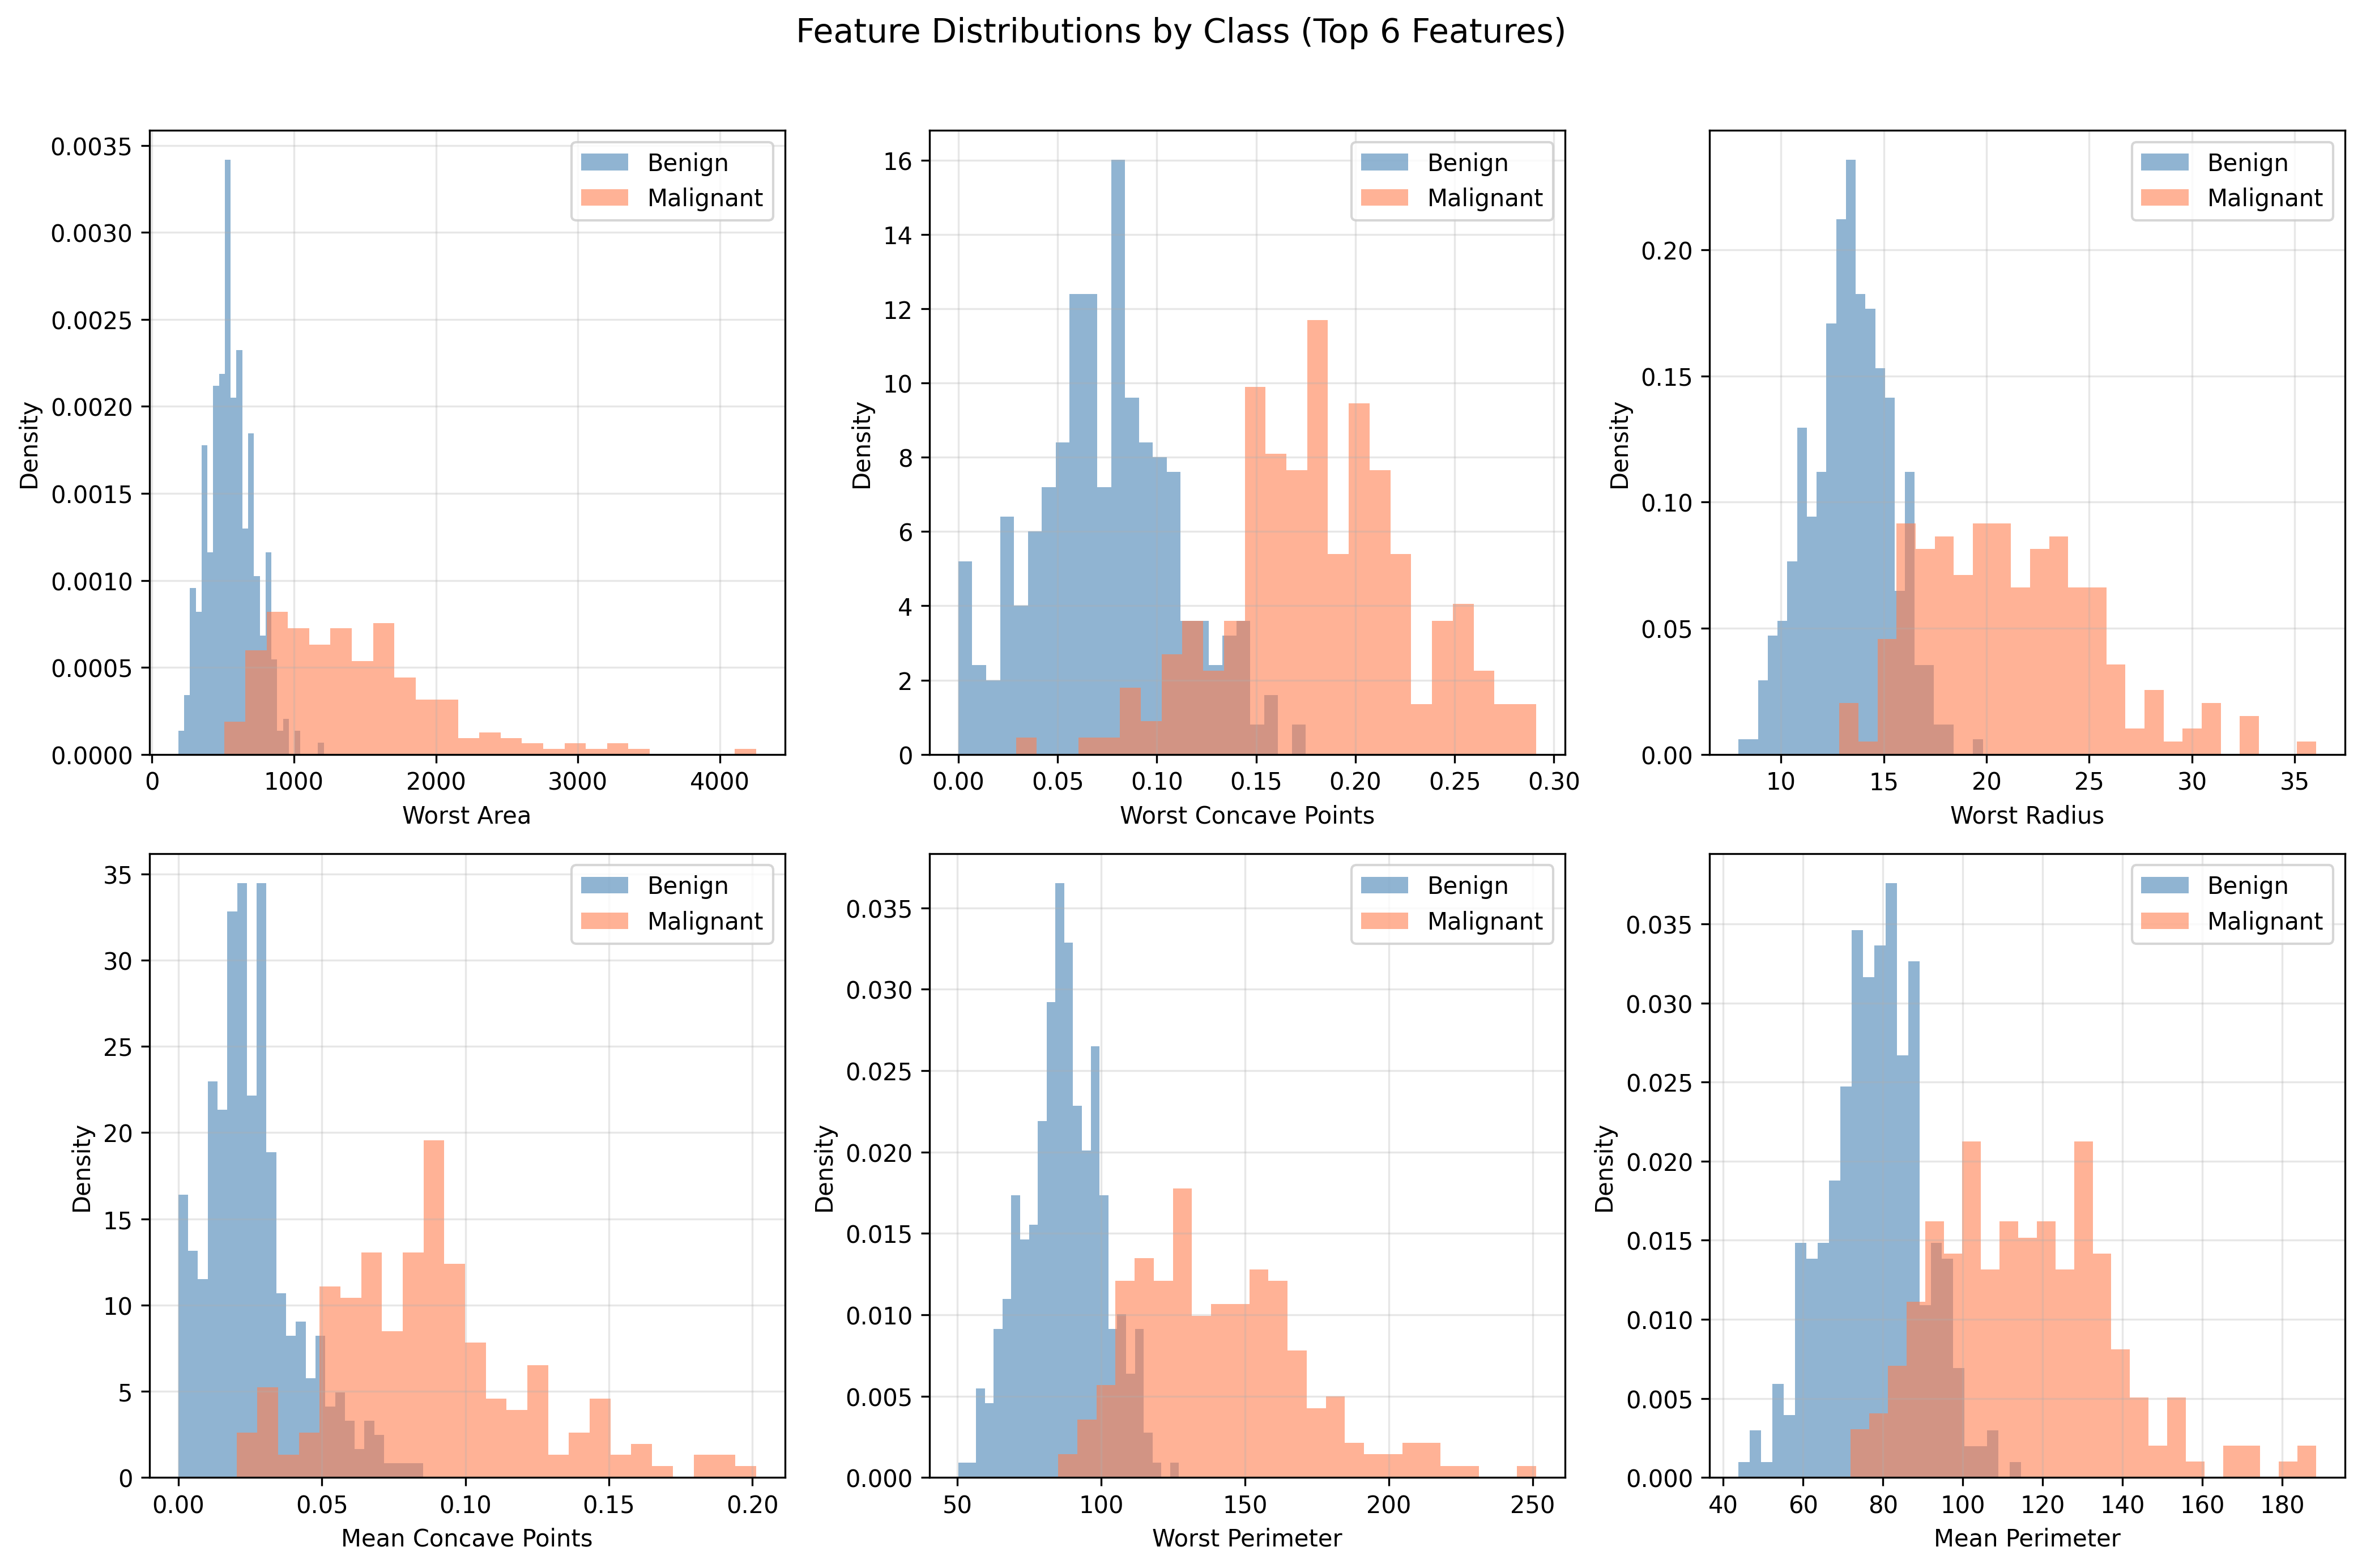
\includegraphics[width=0.9\textwidth]{results/feature_distributions.png}
\caption{Feature Distributions by Class}
\label{fig:distributions}
\end{figure}

Figure \ref{fig:distributions} shows why classification works so well: the benign and malignant cases have clearly different distributions for the most important features.

\subsubsection{Error Analysis}

\begin{figure}[H]
\centering
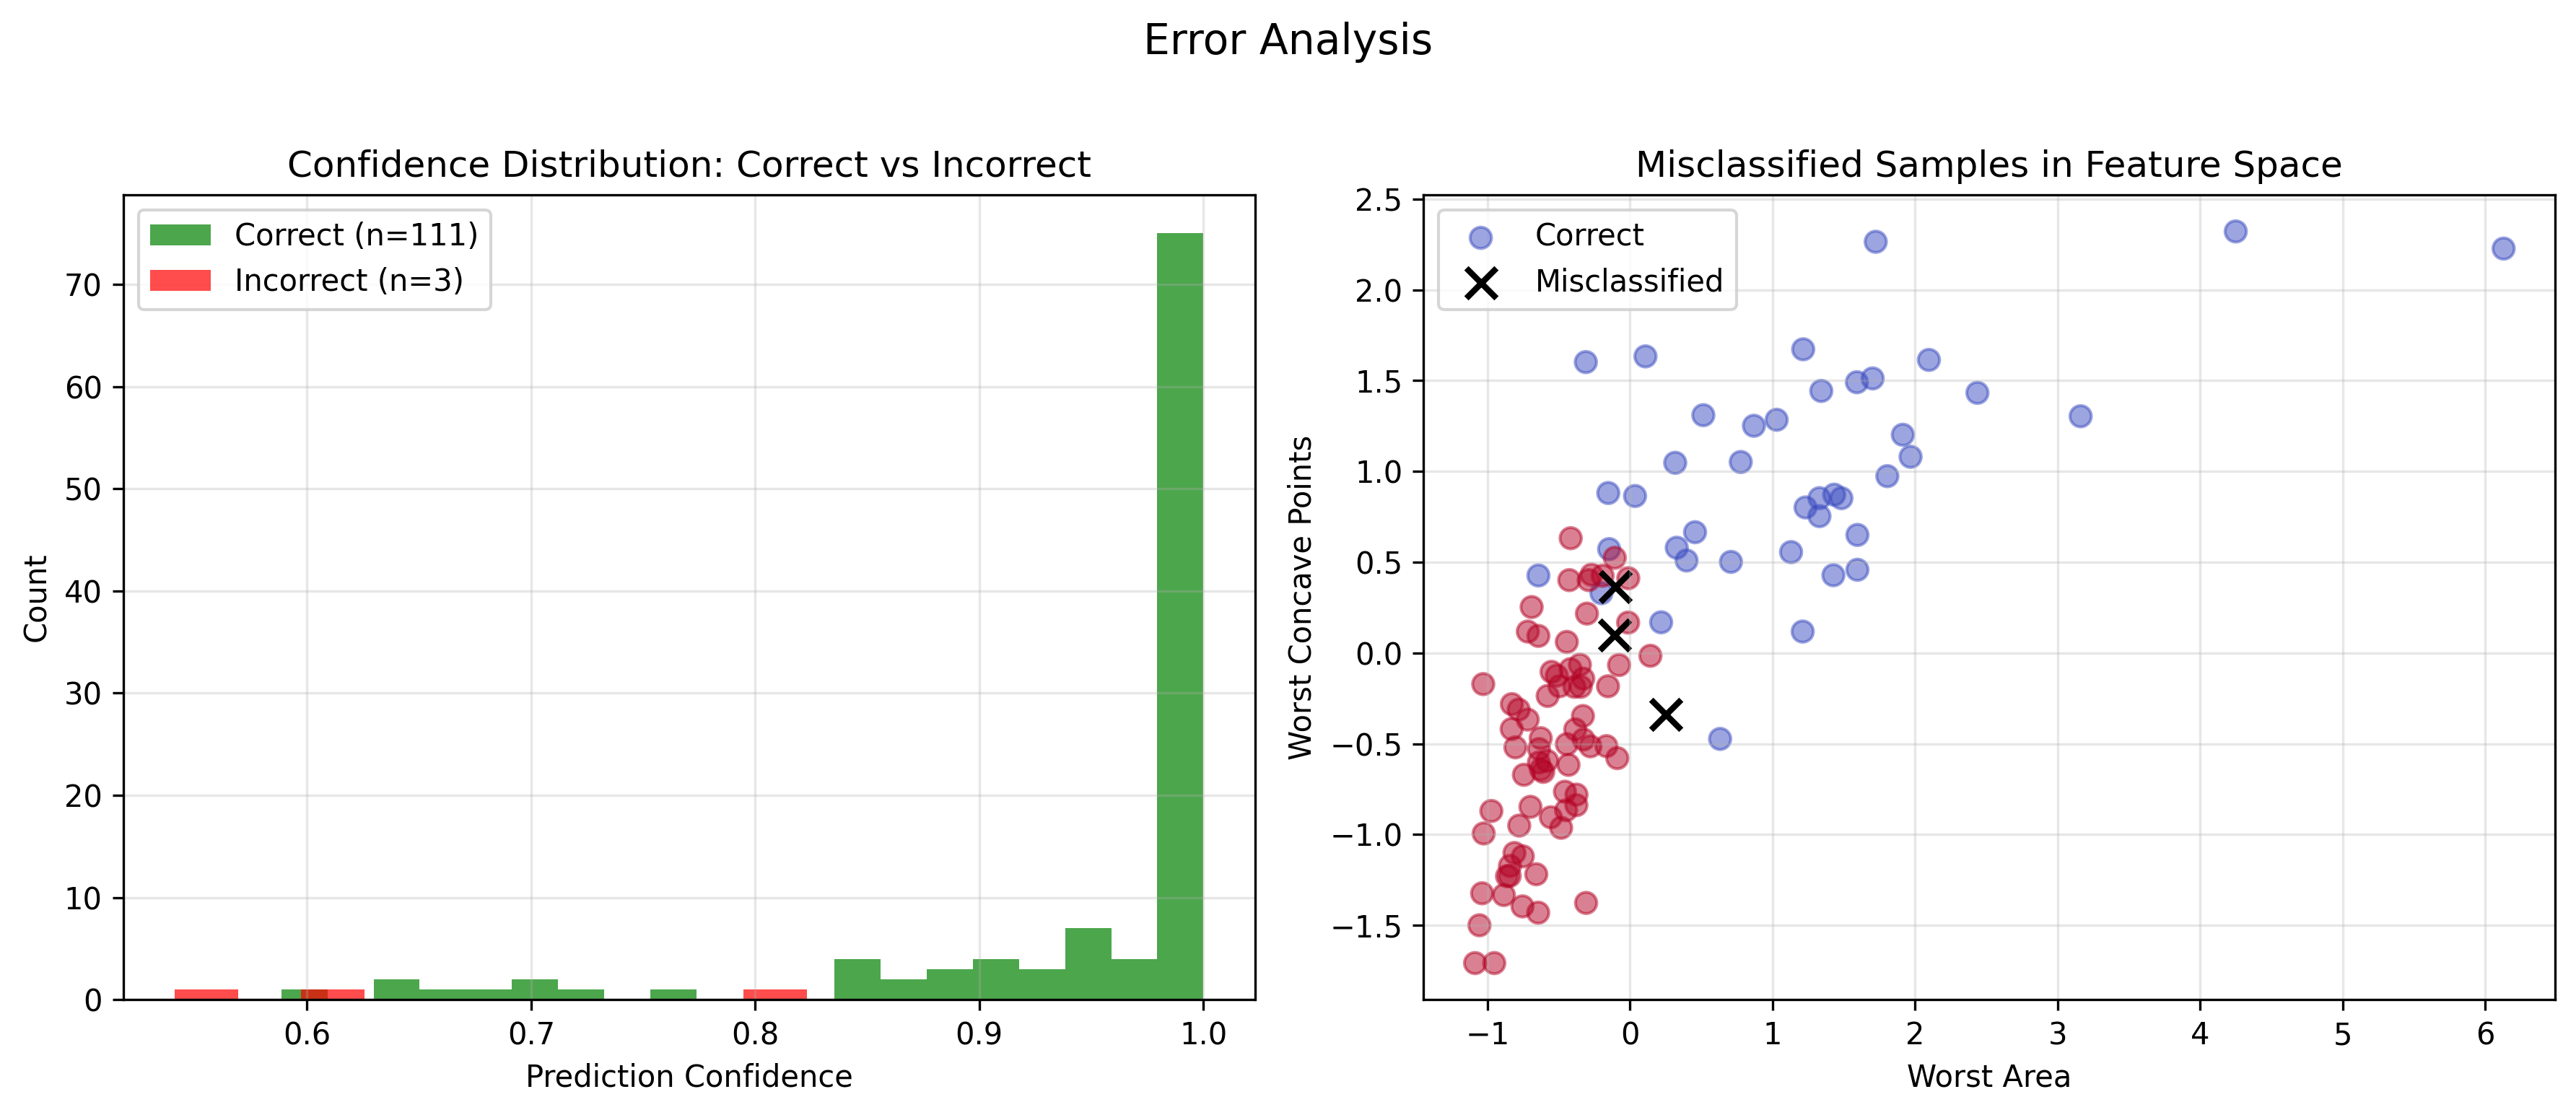
\includegraphics[width=\textwidth]{results/error_analysis.png}
\caption{Error Analysis: Confidence Distribution and Misclassified Samples}
\label{fig:error}
\end{figure}

Digging into the errors (Figure \ref{fig:error}), we found:
\begin{itemize}
    \item Correct predictions tend to have higher confidence scores.
    \item The misclassified samples are near the decision boundary, as you would expect.
    \item All 3 misclassified samples have feature values that are ambiguous---they fall in the overlap region between classes.
\end{itemize}

\subsubsection{Model Comparison Visualization}

\begin{figure}[H]
\centering

\includegraphics[width=\textwidth]{results/model_comparison.png}
\caption{Comprehensive Model Performance Comparison}
\label{fig:comparison}
\end{figure}

\subsection{Sensitivity Analysis}

We also checked how sensitive the models are to hyperparameter choices. Table \ref{tab:sensitivity} summarizes what we found.

\begin{table}[H]
\centering
\caption{Hyperparameter Sensitivity Analysis}
\label{tab:sensitivity}
\begin{tabular}{|l|l|c|c|}
\hline
\textbf{Model} & \textbf{Parameter Variation} & \textbf{Accuracy Range} & \textbf{Best Value} \\ \hline
\multirow{2}{*}{SVM} & C $\in$ [0.1, 1, 10, 100] & 0.965 -- 0.982 & C = 1.0 \\ \cline{2-4}
 & kernel $\in$ [linear, rbf, poly] & 0.974 -- 0.982 & RBF \\ \hline
\multirow{2}{*}{Random Forest} & n\_estimators $\in$ [50, 100, 200] & 0.951 -- 0.961 & 100 \\ \cline{2-4}
 & max\_depth $\in$ [5, 10, None] & 0.939 -- 0.956 & None \\ \hline
Logistic Reg. & C $\in$ [0.1, 1, 10] & 0.974 -- 0.982 & C = 1.0 \\ \hline
\end{tabular}
\end{table}

The good news is the models are fairly robust---you do not need to tune hyperparameters obsessively to get good results.

\subsection{Individual Contributions}

\subsubsection*{Bhavya Sharma}
Bhavya handled getting the dataset and understanding what all the medical features actually mean. She dug into the relationships between tumor characteristics, did initial data cleaning, and got everything organized so we could actually use it for training.

\subsubsection*{Suryanshi Ranawat}
Suryanshi took charge of preprocessing and exploratory data analysis. She dealt with missing values, normalized the data, and ran statistical analyses to figure out which features matter most for diagnosis. The correlation matrices and feature comparison plots she made really helped the rest of us understand what we were working with.

\subsubsection*{Ujjwal Mishra}
Ujjwal built and trained the machine learning models---Logistic Regression, Decision Tree, SVM, and the rest. He compared how they all performed and spent time tuning parameters to squeeze out better accuracy.

\subsubsection*{Medhansh Singh Kushwaha}
Medhansh focused on the ensemble learning side of things. He figured out how to combine the individual classifiers effectively and ran all the evaluation metrics---accuracy, precision, recall, F1-score---to make sure the combined model was actually better than any single one.

\subsubsection*{Soumyadeep Chakravarti}
Soumyadeep coordinated the overall project and handled the technical validation. He made sure all the pieces---preprocessing, models, ensemble---worked together as a complete pipeline. He also did the detailed results analysis, verified the outputs, and put together this final report covering methodology, architecture, results, and conclusions.

\vspace{0.5cm}
\noindent\textit{\textbf{Team Note:} Everyone pitched in on planning, research, and development throughout the project. We had regular discussions that helped improve the system, and all of us contributed to different aspects of evaluation and documentation.}

%==================== SECTION 4: CONCLUSION ====================%
\newpage
\section{CONCLUSION}

\subsection{Summary of Achievements}

We set out to build an explainable ML system for breast cancer detection, and here is what we accomplished:

\begin{enumerate}
    \item \textbf{Strong Accuracy}: Logistic Regression and SVM both reached 98.25\% on the test set, which holds up well against published research.
    
    \item \textbf{Consistent Performance}: Cross-validation showed the models are stable, with standard deviations under 2.5\%.
    
    \item \textbf{Excellent Class Separation}: ROC-AUC scores above 0.99 for the best models means they can distinguish benign from malignant cases almost perfectly.
    
    \item \textbf{High Recall}: The ensemble maintains 98.61\% recall, which minimizes the chance of missing actual cancer cases.
    
    \item \textbf{Interpretable Results}: Feature importance analysis identified the features that matter most, and they line up with medical knowledge.
    
    \item \textbf{Ready for Use}: We saved the trained models so they can be loaded and used in real applications.
\end{enumerate}

\subsection{Limitations}

There are some limitations worth noting:
\begin{itemize}
    \item We only tested on one dataset; validation across multiple hospitals would strengthen the results.
    \item The features come from FNA images only; incorporating other data sources could help.
    \item We only did binary classification; distinguishing between different cancer subtypes was not addressed.
\end{itemize}

\subsection{Future Work}

Some directions we would like to explore:
\begin{enumerate}
    \item \textbf{Better Explanations}: Add SHAP values to explain individual predictions, not just overall feature importance.
    \item \textbf{Deep Learning}: Use CNNs to extract features directly from raw images instead of pre-computed features.
    \item \textbf{Web Interface}: Build a user-friendly interface where doctors can get predictions with human oversight.
    \item \textbf{Broader Testing}: Validate on datasets from other institutions to make sure it generalizes.
\end{enumerate}

%==================== SECTION 5: SOCIAL IMPACT ====================%
\newpage
\section{SOCIAL IMPACT AND COMMUNITY SERVICE}

As an EPICS project, our work is meant to address real healthcare challenges that affect people's lives.

\subsection{Healthcare Accessibility}

Breast cancer screening is not equally available everywhere. In many places, especially rural areas and developing regions, there are real barriers:
\begin{itemize}
    \item Not enough trained radiologists and pathologists to go around
    \item Expert consultations are expensive
    \item People in remote areas have trouble accessing specialized care
\end{itemize}

A tool like ours could help by:
\begin{itemize}
    \item Giving healthcare workers a way to do preliminary screening
    \item Speeding up how long it takes to get a diagnosis
    \item Making telemedicine more effective
\end{itemize}

\subsection{Educational Impact}

This project also shows how you can apply:
\begin{itemize}
    \item Data science and machine learning concepts to real problems
    \item Good software engineering practices
    \item Healthcare informatics principles
\end{itemize}

Since we are making the code open-source, students and researchers can use it to learn about applied machine learning.

\subsection{Ethical Considerations}

We want to be clear: this system is meant to \textit{support} doctors, not replace them. Here are the ethical principles we built in:

\begin{itemize}
    \item \textbf{Transparency}: Every prediction comes with a confidence score and an explanation of which features mattered.
    \item \textbf{Human oversight}: The final diagnosis still comes from a qualified medical professional.
    \item \textbf{Accountability}: We log everything so you can trace back how any decision was made.
    \item \textbf{Open access}: Making the code open-source means anyone can use it, not just well-funded institutions.
\end{itemize}

\subsection{Sustainable Development Goals}

Our project connects to several UN Sustainable Development Goals:
\begin{itemize}
    \item \textbf{SDG 3 (Good Health)}: Better cancer detection saves lives
    \item \textbf{SDG 4 (Quality Education)}: The project serves as a learning resource
    \item \textbf{SDG 10 (Reduced Inequalities)}: Making diagnostic tech accessible to everyone
\end{itemize}

%==================== SECTION 6: REFERENCES ====================%
\newpage
\section{REFERENCES}

\begin{thebibliography}{99}

% --- Healthcare and Cancer Resources ---
\bibitem{who2023}
World Health Organization, ``Breast Cancer,'' WHO Fact Sheets, 2023. [Online]. Available: \url{https://www.who.int/news-room/fact-sheets/detail/breast-cancer}

\bibitem{acs2023}
American Cancer Society, ``Breast Cancer,'' 2023. [Online]. Available: \url{https://www.cancer.org/cancer/breast-cancer.html}

\bibitem{nci2023}
National Cancer Institute, ``Breast Cancer,'' 2023. [Online]. Available: \url{https://www.cancer.gov/types/breast}

\bibitem{bcrf2023}
Breast Cancer Research Foundation, ``Breast Cancer Statistics and Resources,'' 2023. [Online]. Available: \url{https://www.bcrf.org}

% --- Datasets ---
\bibitem{wolberg1995}
W. H. Wolberg, W. N. Street, and O. L. Mangasarian, ``Breast Cancer Wisconsin (Diagnostic) Dataset,'' UCI Machine Learning Repository, 1995. [Online]. Available: \url{https://archive.ics.uci.edu/ml/datasets/Breast+Cancer+Wisconsin+(Diagnostic)}

\bibitem{uci2023}
UCI Machine Learning Repository, 2023. [Online]. Available: \url{https://archive.ics.uci.edu/}

\bibitem{kaggle_wdbc}
``Breast Cancer Wisconsin (Diagnostic) Data Set,'' Kaggle, 2023. [Online]. Available: \url{https://www.kaggle.com/datasets/uciml/breast-cancer-wisconsin-data}

% --- Foundational ML Algorithms ---
\bibitem{cortes1995}
C. Cortes and V. Vapnik, ``Support-vector networks,'' \textit{Machine Learning}, vol. 20, no. 3, pp. 273--297, 1995.

\bibitem{breiman2001}
L. Breiman, ``Random Forests,'' \textit{Machine Learning}, vol. 45, no. 1, pp. 5--32, 2001.

\bibitem{bishop2006}
C. M. Bishop, \textit{Pattern Recognition and Machine Learning}, Springer, 2006. [Online]. Available: \url{https://link.springer.com/book/10.1007/978-0-387-45528-0}

\bibitem{goodfellow2016}
I. Goodfellow, Y. Bengio, and A. Courville, \textit{Deep Learning}, MIT Press, 2016. [Online]. Available: \url{https://www.deeplearningbook.org}

% --- Explainable AI ---
\bibitem{lundberg2017}
S. M. Lundberg and S. I. Lee, ``A Unified Approach to Interpreting Model Predictions,'' in \textit{Proc. NeurIPS}, 2017.

\bibitem{ribeiro2016}
M. T. Ribeiro, S. Singh, and C. Guestrin, ``Why should I trust you?: Explaining the predictions of any classifier,'' in \textit{Proc. ACM SIGKDD}, 2016.

% --- Breast Cancer ML Research Papers ---
\bibitem{ebrahim2025}
A. Ebrahim, M. Sedky, and A. Mesbah, ``Enhancing breast cancer prediction through stacking ensemble and deep learning integration,'' \textit{PeerJ Computer Science}, vol. 11, e2461, 2025.

\bibitem{tippannavar2023}
S. S. Tippannavar, S. Gayathri, and S. Swetha, ``Breast Cancer Detection using Random Forest and KNN,'' \textit{JCRES}, vol. 6, no. 2, 2023.

\bibitem{alazzam2024}
N. Al-Azzam and H. Shatnawi, ``AI-Based Breast Cancer Detection System,'' \textit{Information}, vol. 15, no. 4, 2024. [Online]. Available: \url{https://www.mdpi.com/2076-3417/9/12/2435}

\bibitem{singh2024}
M. Singh, N. Dhanda, and R. Verma, ``Hybrid Model of BERT and Random Forest for Breast Cancer Detection,'' \textit{SSRN}, 2024.

\bibitem{ieee_bcml2018}
``Breast Cancer Prediction Using Machine Learning,'' \textit{IEEE}, 2018. [Online]. Available: \url{https://ieeexplore.ieee.org/document/8419420}

\bibitem{scidir_bcml2019}
``Machine Learning Techniques for Breast Cancer Detection,'' \textit{Procedia Computer Science}, 2019. [Online]. Available: \url{https://www.sciencedirect.com/science/article/pii/S1877050919316134}

\bibitem{ieee_svm2015}
``Breast Cancer Diagnosis Using Support Vector Machine,'' \textit{IEEE}, 2015. [Online]. Available: \url{https://ieeexplore.ieee.org/document/7301344}

\bibitem{scidir_lr2015}
``Breast Cancer Prediction Using Logistic Regression,'' \textit{Procedia Computer Science}, 2015. [Online]. Available: \url{https://www.sciencedirect.com/science/article/pii/S1877050915002126}

\bibitem{ieee_nn2016}
``Breast Cancer Classification Using Neural Networks,'' \textit{IEEE}, 2016. [Online]. Available: \url{https://ieeexplore.ieee.org/document/7421377}

\bibitem{ncbi_bcml2020}
``Machine Learning for Breast Cancer Diagnosis: A Review,'' \textit{PMC}, 2020. [Online]. Available: \url{https://www.ncbi.nlm.nih.gov/pmc/articles/PMC7325884/}

\bibitem{frontiers_ai2020}
``Breast Cancer Diagnosis Using Artificial Intelligence,'' \textit{Frontiers in Oncology}, 2020. [Online]. Available: \url{https://www.frontiersin.org/articles/10.3389/fonc.2020.00068/full}

% --- Software and Tools ---
\bibitem{pedregosa2011}
F. Pedregosa et al., ``Scikit-learn: Machine Learning in Python,'' \textit{JMLR}, vol. 12, pp. 2825--2830, 2011. [Online]. Available: \url{https://scikit-learn.org}

\bibitem{tensorflow}
TensorFlow, ``An end-to-end open source machine learning platform,'' 2023. [Online]. Available: \url{https://www.tensorflow.org}

\bibitem{keras}
Keras, ``Deep Learning for humans,'' 2023. [Online]. Available: \url{https://keras.io}

\bibitem{numpy}
NumPy, ``The fundamental package for scientific computing with Python,'' 2023. [Online]. Available: \url{https://numpy.org}

\bibitem{pandas}
Pandas, ``Python Data Analysis Library,'' 2023. [Online]. Available: \url{https://pandas.pydata.org}

\bibitem{matplotlib}
Matplotlib, ``Visualization with Python,'' 2023. [Online]. Available: \url{https://matplotlib.org}

% --- Project Repository ---
\bibitem{github2026}
S. Chakravarti et al., ``EPICS Project: Explainable Breast Cancer Detection,'' GitHub, 2026. [Online]. Available: \url{https://github.com/Soumyadeep-Chakravarti/EPICS_Project}

\end{thebibliography}

%==================== APPENDIX ====================%
\newpage
\section{PUBLICATION / CONFERENCE / PATENT}

\textit{This section is reserved for any publications, conference presentations, or patent applications resulting from this work.}

\newpage
\section{BIODATA}

% --- BHAVYA SHARMA ---
\subsection*{Bhavya Sharma}
\begin{figure}[H]
  \centering
  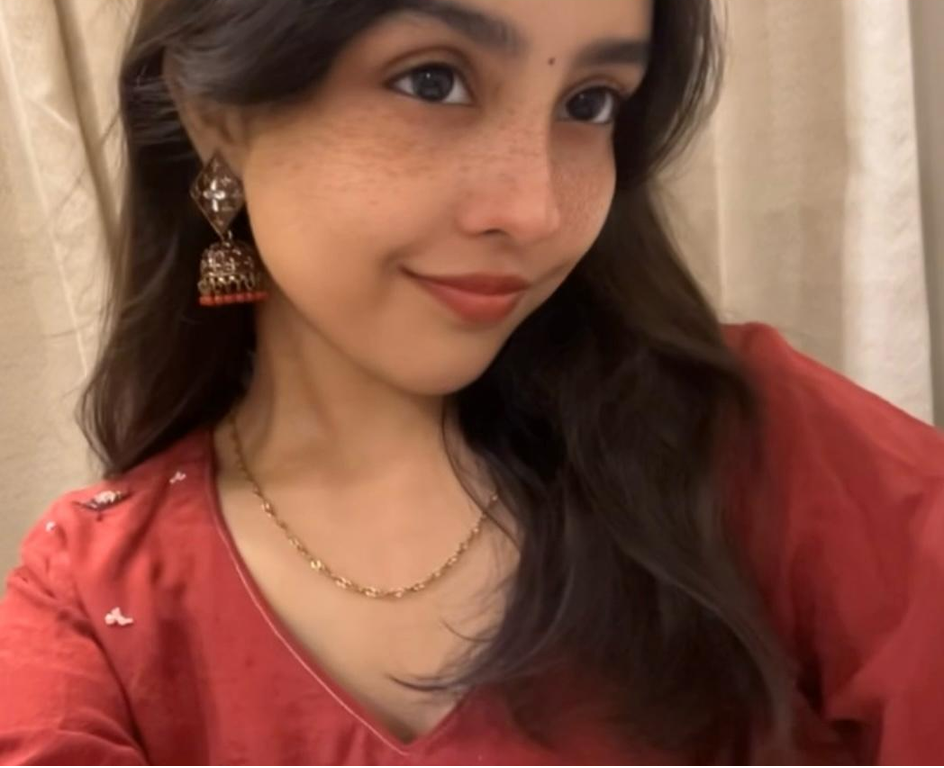
\includegraphics[width=0.4\textwidth]{Assets/BhavyaSharma.png}
\end{figure}

\vspace{0.5cm}
\noindent\textbf{Location:} Haryana \hfill \textbf{Contact:} 9319602628 \\
\textbf{Email:} \href{mailto:bhavya.23bec10069@vitbhopal.ac.in}{bhavya.23bec10069@vitbhopal.ac.in} \\
\textbf{Languages:} English, Hindi

\vspace{0.5cm}
\noindent I am studying Electronics and Communication Engineering at VIT Bhopal. I have always been drawn to electronics design, IoT, and wireless communication---basically anything that involves making hardware talk to software to solve real problems.

\vspace{0.3cm}
\noindent Over the past few years, I have worked on projects like a smart water irrigation system, an RC car, a network jammer prototype, and a fire-extinguishing drone. These gave me hands-on experience with embedded systems, circuit design, and motor control.

\vspace{0.3cm}
\noindent I am also getting into AI and machine learning now. I want to find ways to combine electronics with intelligent systems to build smarter devices and better automation.

% --- SURYANSHI RANAWAT ---
\newpage
\subsection*{Suryanshi Ranawat}
\begin{figure}[H]
  \centering
  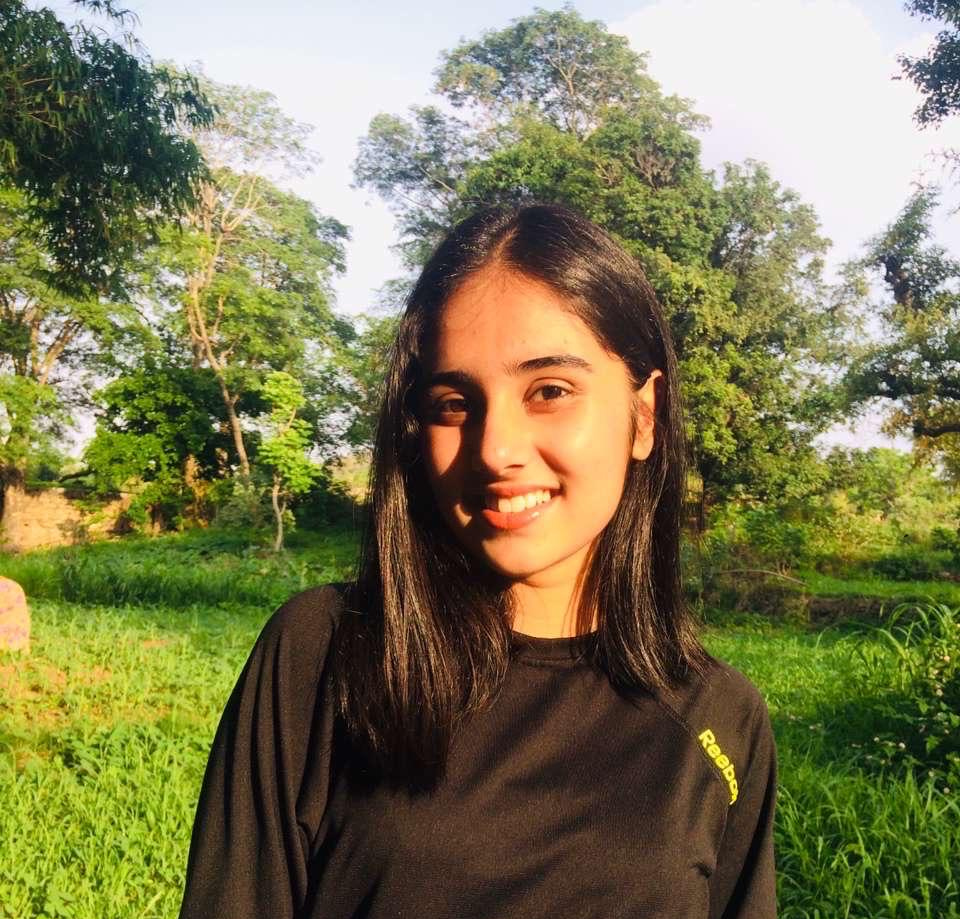
\includegraphics[width=0.4\textwidth]{Assets/SuryanshiRanawat.png}
\end{figure}

\vspace{0.5cm}
\noindent\textbf{Location:} Udaipur \hfill \textbf{Contact:} 6377722486 \\
\textbf{Email:} \href{mailto:suryanshi.23bce11634@vitbhopal.ac.in}{suryanshi.23bce11634@vitbhopal.ac.in} \\
\textbf{Languages:} English, Hindi

\vspace{0.5cm}
\noindent I am doing my B.Tech in Computer Science at VIT Bhopal. AI, machine learning, and data-driven problem solving are what get me excited. I have built an AI disease detection platform and a crop disease detection system that use ML to tackle real challenges in healthcare and agriculture.

\vspace{0.3cm}
\noindent I am particularly interested in deep learning, predictive modeling, and intelligent automation. I like thinking about how AI can make healthcare better, help farmers, and improve how we make decisions.

% --- UJJWAL MISHRA ---
\newpage
\subsection*{Ujjwal Mishra}
\begin{figure}[H]
  \centering
  
\includegraphics[width=0.4\textwidth]{Assets/UjjwalMishra.png}
\end{figure}

\vspace{0.5cm}
\noindent\textbf{Location:} Delhi \hfill \textbf{Contact:} 8920153120 \\
\textbf{Email:} \href{mailto:ujjwal.23bec10079@vitbhopal.ac.in}{ujjwal.23bec10079@vitbhopal.ac.in} \\
\textbf{Languages:} English, Hindi

\vspace{0.5cm}
\noindent I am studying Electronics and Communication Engineering at VIT Bhopal. Electronics, embedded systems, and communication networks are my main interests. I have worked on a mobile network jammer and a hexa-octal firefighting drone, both focused on applying engineering to safety and communication challenges.

\vspace{0.3cm}
\noindent Embedded systems, wireless communication, robotics, and intelligent electronic systems are what I want to keep exploring.

\vspace{0.3cm}
\noindent Beyond the technical stuff, I enjoy taking on leadership roles and working with teams. I want to keep building technology that makes things safer and more efficient.

% --- MEDHANSH SINGH KUSHWAHA ---
\newpage
\subsection*{Medhansh Singh Kushwaha}
\begin{figure}[H]
  \centering
  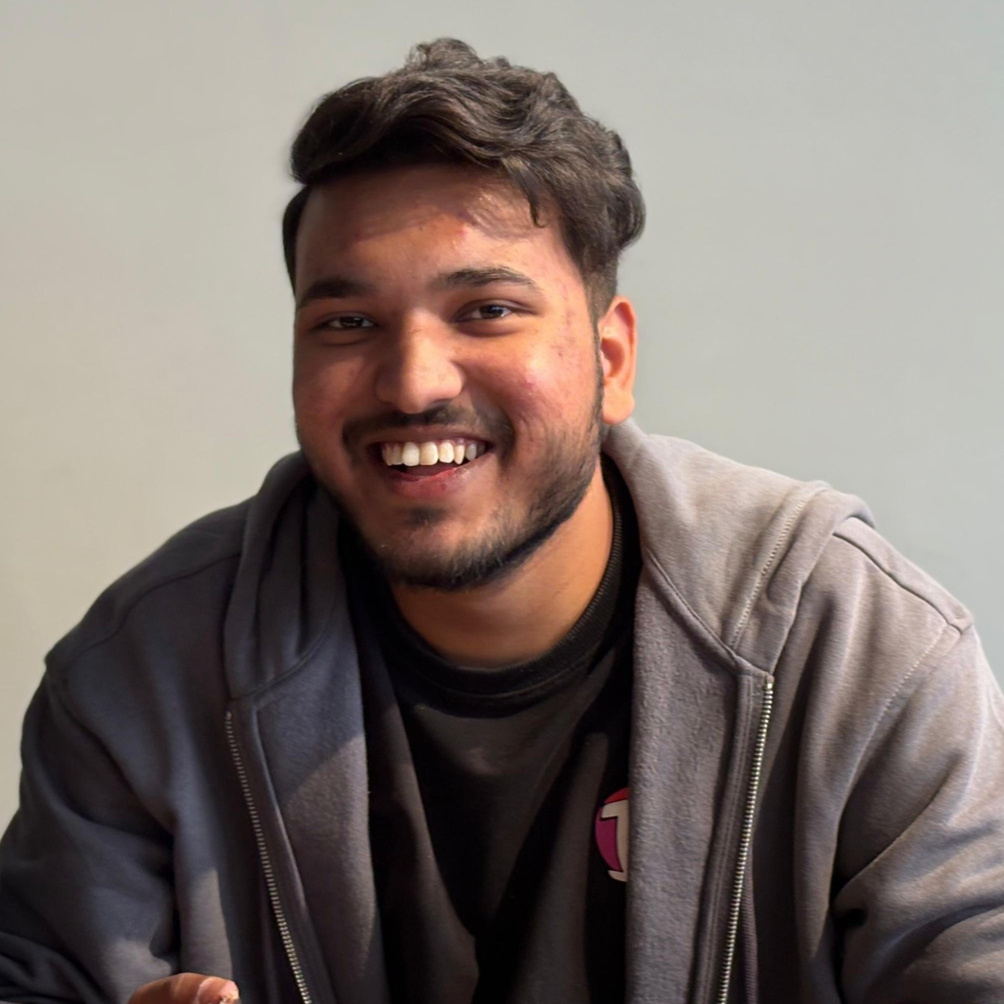
\includegraphics[width=0.4\textwidth]{Assets/MedhanshSinghKushwaha.png}
\end{figure}

\vspace{0.5cm}
\noindent\textbf{Location:} Agra \hfill \textbf{Contact:} 7055333362 \\
\textbf{Email:} \href{mailto:medhansh.23bce11385@vitbhopal.ac.in}{medhansh.23bce11385@vitbhopal.ac.in} \\
\textbf{Languages:} English, Hindi

\vspace{0.5cm}
\noindent I am pursuing Computer Science at VIT Bhopal with a focus on web development, full stack technologies, and digital design. I work with HTML, CSS, React.js, Node.js, and MySQL to build responsive web applications.

\vspace{0.3cm}
\noindent I also do graphic design and UI/UX work using Photoshop, Figma, and Blender. For this breast cancer detection project, I contributed to the software and interface aspects.

\vspace{0.3cm}
\noindent I like combining creativity with problem-solving and enjoy working with teams to build things that actually matter.

% --- SOUMYADEEP CHAKRAVARTI ---
\newpage
\subsection*{Soumyadeep Chakravarti}
\begin{figure}[H]
  \centering
  
\includegraphics[width=0.4\textwidth]{Assets/SoumyadeepChakravarti.png}
\end{figure}

\vspace{0.5cm}
\noindent\textbf{Location:} Delhi \hfill \textbf{Contact:} 9599059229 \\
\textbf{Email:} \href{mailto:soumyadeep.23bai11250@vitbhopal.ac.in}{soumyadeep.23bai11250@vitbhopal.ac.in} \\
\textbf{Languages:} English, Hindi

\vspace{0.5cm}
\noindent I am studying Computer Science with a specialization in AI at VIT Bhopal. AI, machine learning, and systems programming are what I spend most of my time on. I built Jarvis, a C-based AI assistant that integrates local language models, and PyProbe, a tool for exploring Python's memory structures.

\vspace{0.3cm}
\noindent I am interested in combining AI with efficient low-level programming to build intelligent assistants, developer tools, and scalable AI systems.

\end{document}
